\documentclass[11pt]{book}
\usepackage[utf8]{inputenc}
\usepackage[T1]{fontenc}
\usepackage[numbers]{natbib}
\usepackage[mode=buildmissing]{standalone}
\usepackage{tikz}
\usepackage{graphicx}
\usepackage{hyperref}
\usepackage{cleveref}
\usepackage{subcaption}
\usepackage{minted}
\usepackage{csquotes}
\usepackage{multirow}
\usepackage{tabularx}
\usepackage{tikz-uml}
\usepackage{threeparttable}
\usepackage[]{siunitx}
\usepackage{makecell}
\usepackage{graphbox}
\usepackage[draft]{fixme}
\usepackage{makecell}
\usepackage{bibentry}
\usepackage{amsfonts}
\usepackage{amssymb}
\usepackage{svg}

\usepackage[section]{placeins}

\usepackage{pifont}
\newcommand{\cmark}{\ding{51}}%
\newcommand{\xmark}{\ding{55}}%
\newcommand{\eqmark}{{\bf $\approx$}}

\definecolor{lightgray}{rgb}{0.83, 0.83, 0.83}
\definecolor{lightblue}{rgb}{0.68, 0.85, 0.9}
\definecolor{lightgreen}{rgb}{0.56, 0.93, 0.56}
\definecolor{thistle}{rgb}{0.85, 0.75, 0.85}

\newcommand{\FIXME}[1]{{\color{red}#1}}
\newcommand{\PLAGIAT}[1]{{\color{magenta}#1}}

% Reset chapter number after each part
\makeatletter
\@addtoreset{chapter}{part}
\makeatother  

%\renewcommand{\baselinestretch}{1} 

\usetikzlibrary{3d,calc,positioning}
\tikzumlset{font=\scriptsize\tt}
\setminted{fontsize=\scriptsize}

\renewcommand\UrlFont{\color{blue}\rmfamily}

\begin{document}
%
\title{Programming in modern C++ for image processing}


\author{Michaël Roynard}

%\institute{EPITA Research and Development Laboratory\\
%  \email{michael.roynard@lrde.epita.fr}
%}


\maketitle

\section{Acknowledgement}
\label{sec.acknowledgement}


\section{Abstract}
\label{sec.abstract}
TODO EN

TODO FR

\section{Long abstract}
\label{sec.long_abstract}


\tableofcontents
\label{table.of.contents}

\listoffigures
\label{list.of.figures}

\listoftables
\label{list.of.tables}

\cleardoublepage


\part{Introduction}
\label{part.introduction}

\chapter{Introduction}
\label{chap:introduction}

\section*{Outline}

\lettrine[lines=2]{N}{owadays} \emph{Computer Vision} and \emph{Image Processing (IP)} are omnipresent in the day to day
life of the people. It is present each time we pass by a CCTV camera, each time we go to the hospital do an MRI, each
time we drive our car and pass in front of a speed camera and each time we use our computer, smartphone or tablet. We
just cannot avoid it anymore. The systems using this technology are sometimes simple and, sometimes, more complex. Also
the usage made of this technology has several different purposes: space observation, medical, quality of life
improvement, surveillance, control, autonomous system, etc. Henceforth, Image processing has a wide range of research
and despite having a mass of previous of work already contributed to, there are still a lot to explore.

Let us take the example of a modern smartphone application which provides facial recognition in order to recognize
people whom are featuring inside a photo. To provide accurate result, this application will have to do a lot of
different processing. Indeed, there are a lot of elements to handle. We can list (non exhaustively) the weather, the
light exposition, the resolution, the orientation, the number of person, the localization of the person, the distinction
between humans and objects/animals, etc. All of these is in order to finally recognizing the person(s) inside the photo.
What the application does not tell you is the complexity of the image processing pipeline behind the scene that can not
even be executed in its entirety on one's device (smartphone, tablet, \ldots). Indeed, image processing is costly in
computing ressources and would not meet the time requirement desired by the user if the entire pipeline was executed on
the device. Furthermore, for the final part which is "recognize the person on the photo", one needs to feed the
pre-processed photo to a neural network trained beforehand through deep learning techniques in order to give an accurate
response. There exists technologies able to embed neural network into mobile phone such as
MobileNets~\parencite{howard.2017.mobilenets} but it is still limited. It can detect a human being inside a photo but
not give the answer about who this human being is for instance. That is why, accurate neural network system usually are
abstracted away in cloud technologies making them available only via Internet. When uploading his image, the user does
not imagine the amount of technologies and computing power that will be used to find who is on the photo.

We now understand that in order to build applications that interact with photos or videos nowadays, we need to be able
to do accurate, fast and scalable image processing on a multitude of devices (smartphone, tablet, \ldots). In order to
achieve this goal, image processing practitioners needs to have two kinds of tools at their disposal. One will be the
prototyping environnement, a toolbox which allow the practitioner to develop, test and improve its application logic.
The other is the production environnement which deploy the viable version of the application that was developed by the
practitioner. Both environment may not have the same needs. On one hand, the prototyping environment usually requires to
have a fast feedback loop for testing, an availability of state-of-the-art algorithms and existing software. This way
the practitioner can easily build upon them and be fast enough in order not to keep waiting for results when testing
many prototypes. On the other hand, the production environment must be stable, resilient, fast and scalable.

When looking at standards in the industry nowadays, we notice that Python is the main choice for prototyping. Also,
Python may not be enough so that a viable prototype can be pushed in production with minimal changes afterwards. We find
it non-ideal that the practitioner cannot take advantages of many optimisation opportunities, both in term of algorithm
efficiency and better hardware usage, when proceeding this way. It would be much more efficient to have basic low level
building blocks that can be adapted to fit as mush use cases as possible. This way, the practitioner can easily build
upon them when designing its application. We distinguishes two kind of use cases. The first one is about the
multiplicity of types or algorithms the practitioner is facing. The second one is about the diversity of hardware the
practitioner may want to run his program. The goal is to have building blocks that can be intelligent enough to take
advantage of many optimization opportunities, with regard to both input data types/algorithms and target hardware. Then
the practitioner would have a huge performance improvement, by default, without specifically tweaking its application.
As such, the concept of genericity was introduced. It aims at providing a common ground about how an image should behave
when passed to basic algorithms needed for complex applications. This way, in theory, one only needs to write the
algorithm once for it to work with any given kind of image.


\section*{Different data types and algorithms}

In Image Processing, there exists a multitude of image types whose characteristics can be vastly different from one
another. This large specter is also resulting from the large domain of application of image processing. For instance,
when considering photography we have 2D image whose values can vary from 8 bits grayscale to multiple band 32-bits color
scheme storing informations about the non-visible specter of human eye. If we consider another domain of application,
such as medical imaging, we now can consider sequence of images such as sequence of 3D image for an MRI for instance.
More broadly there are two orthogonal constituent of an image: its topology (or structure) and its values. However,
there are two more aspectes to consider here. Firstly, image processing provide plenty of algorithms that can or cannot
operate over specific data types. There are also different kind of algorithms. Some will extract informations,(e.g.
histogram) other will transform the image point-wise (e.g. thresholding), and some other will even combine several image
to render a different kind of informations (e.g. background substraction). There are many simple algorithms and also
many complex algorithms out there. Secondly, there are orbiting data around image types and algorithms that are also
very diverse and necessary for their smooth operation. Indeed, a dilation algorithm will also need an additional
information: the dilation disc. A thresholding algorithm may be given a threshold. A convolution filter requires a
convolution matrix to operate. That is why, when considering both image types and algorithms, we need a 3D-chart
(illustrated in~\cref{fig:int.possibility_space}) to enumerate all possibilities, where one axis is the image topology,
one axis is the color scheme and one axis enumerate the additional data that can be associated to an image.


\begin{figure}[tbh]
  \centering
  \includegraphics{figs/possibility_space}
  \caption{Illustration of the specter of the multitude of possibilities in the image processing world.}
  \label{fig:int.possibility_space}
\end{figure}


\section*{Different user profiles and their use cases}

\paragraph{The end user} is a non programmer user who wants to occasionally use image processing software through
UI-rich interface, such as Adobe Photoshop~\parencite{adobe.2019.photoshop} or The GIMP~\parencite{gimp.2019}. Its
skills are non-relevant as the end user is using the software to get work done even though he does not fully understand
the underlying principles. For instance, the end user will want to correct the brightness of an image, of remove some
impurities from a face or a building. The end user does not want to build an application but wants to save time. The
needs of the end user mainly revolves around a clean and intuitive software UI as well as a well as support for
mainstream image types and operation a photograph may need to do.

\paragraph{The practitioner} is what we are called when we first approach the image processing area. A practitioner is
the end user of image processing libraries. Its skills mainly revolve around applied mathematics for image processing,
prototyping and algorithms. A practitioner aims at leveraging the features the libraries can offer to build his
application. For instance, a practitioner can be a researcher in medical imaging, an engineer build a facial recognition
application, a data scientist labeling its image set, etc. The needs of practitioner are mainly revolving around a fast
feedback loop. The developing environment must be easily accessible and installable. This way a practitioner can judge
quickly wether one library will answer his needs. The documentation of the library must be exhaustive and didactic with
examples. When prototyping, the library must provide fast feedback loops, as in a python notebook for instance. Finally
it must be easily integrated in a standard ecosystem such as being able to work with NumPy's array natively without
imposing its own types. To sum up, practitioner's programmatic skills do not need to be high as his main goal is to
focus on algorithms and mathematics formulas.

\paragraph{The contributer} is an advanced user of a library who is very comfortable with its inner working, philosophy,
aims, strengths and potential shortcomings. As such, he is able to add new specific features to library, fix some
shortcomings or bugs. Usually a contributer is able to add a feature needed for a practitioner to finish his
application. Furthermore he can then contribute back his features to the main project via pull requests if it is
relevant. This way, a maintainer will assess the pull request and review it. The two main points of a contributer are
his deep knowledge of a library and his ability to write code in the same language as the source code of it. Also, a
contributer must have knowledge of coding best practices such as writing unit tests which are mandatory when adding a
feature to an existing library. To facilitate contribution, a library must provide clear guidelines about the way to
contribute, be easy to bootstrap and compile without having heavy requirements on dependencies. The best case would be
that the library is handled by standard packages managers such as system apt or python conan.

\paragraph{The maintainer} is usually the creator, founder of the library or someone that took over the project when the
founder stepped back. Also, when a library grows, it is not rare that regular contributers end up being maintainer as
well to help the project. The maintainer is in charge of keeping alive the project by fulfilling several aspects:
upgrade and release new features according to the user (practitioner) needs and the library philosophy. Also, a library
may not evolve as fast as the user may want it because of lack of time from maintainers. A lot of open source projects
are maintained by volunteers and lack of time is usually the main aspect slowing development progress. The maintainer is
also in charge of reviewing all the contributers pull requests. He must check if they are relevant and completed enough,
(for instance, presence of tests and documentation) to be integrated in the project. Indeed, merging a pull requests
equals to accepting to take care of this code in the future too. It means that further upgrade, bug fix, refactoring of
the project will consider this new code too. If the maintainer is not able to take care of this code then it should
probably not be integrated in the project in the first place. Any project and library has its maintainers. A maintainer
is someone very familiar with the inner working and architectural of the project. He is also someone that has some
history in the project to understand why some decisions has been made, what choices has been made at some points and
what the philosophy of the project is. It is important to be able to refuse a contribution that would go contrary to the
philosophy of the project, even a very interesting one. Finally the profile of a maintainer is one of a developer that
is used to the standard workflow in open source based on: forks, branches, merge/pull requests and continuous
integration.

\section*{Different tools}

Before stating the topic of the thesis, it is important to enumerate the different kind of tools the current market has
to offer to know where we will be positioning ourself.

\paragraph{Graphic editors} are what neophyte thinks about when they imagine what image processing is. Those are tools
that allow a non expert user to apply a wide array of operation on an image from an intuitive GUI in a way the user does
not have to understand the underlying logic behind each and every operation he is applying. Such tools are usually large
complex software such as The GIMP~\parencite{gimp.2019} or Photoshop~\parencite{adobe.2019.photoshop}. Their aim is to
be useable by end users while supporting a large set of popular image format.

\paragraph{Command line utilities} are binaries that perform one operation or more invocable from a console interface or
from a shell script through a command line interface (CLI). This CLI usually offers several options to pass data and/or
information to the programs in order to have an processing happening. The informations can be, for instance, the input
image path, the ouput image name and the name of a mathematical morphology algorithm to apply. Usually command line
utilities come as projects such as ImageMagick~\parencite{imagemagick.2021},
GraphicsMagick~\parencite{graphicsmagick.2021} or MegaWave~\parencite{froment.2012.megawave,froment.2004.megawave2}.

\paragraph{Visual programming environment} are software that allow the user to graphically and intuitively link one or
several image processing operations while interactively displaying the result. The processing can easily be modified and
the results are updated accordingly. Those software are usually aimed at engineer or researchers doing prototyping work
not exclusive to image processing. Mathcad~\parencite{ptc.2019.mathcad} is a good example of such a software.

\paragraph{Integrated environment} are feature-rich platforms for scientists oriented toward prototyping. Those
platforms provides a fully functional programming language and a graphical interface allowing the user to run commands
and scripts as well as viewing results and data (image, matrices, etc.). The most well-known integrated environnement
are Matlab~\parencite{mathworks.2020.matlab}, Scilab~\parencite{scilab.2020}, Octave~\parencite{gnu.2021.octave},
Mathematica~\parencite{wolfram.2020.mathematica} and Jupyter~\parencite{kluyver.2016.jupyter} notebooks.

\paragraph{Package for dynamic language} has known a surge in development these last few years and a multitude of
libraries has been brought to dynamic languages this way. For instance, let us consider the python programming language.
There are two main package provider: PyPi~\parencite{pypi.2021} and Conda~\parencite{anaconda.2020}. Both allow to
install packages to enable the user to program his prototypes in Python very quickly. In image processing, there are
packages such as Scipi~\parencite{jones.2006.scipy}, NumPy~\parencite{oliphant.2006.numpy},
scikit-image~\parencite{vanderWalts.2014.scikit-image}, Pillow~\parencite{clark.2021.pillow} as well as binding for
OpenCV~\parencite{bradski.2000.opencv}.

\paragraph{Programming libraries} is the most common tool available out there. They are a collection of routines,
functions and structures providing features through a documentation and binaries. They require the user to be proficient
with a certain programming language and also to be able to integrate a library into his project. For image processing we
have: IPP~\parencite{taylor.2004.intel}, ITK~\parencite{johnson.2013.ITKSoftwareGuideThirdEdition},
Boost.GIL~\parencite{bourdev.2006.bgil}, Vigra~\parencite{kothe.2011.generic}, GrAL~\parencite{berti.2006.gral},
DGTal~\parencite{coeurjolly.2016.dgtal}, OpenCV~\parencite{bradski.2000.opencv}, CImg~\parencite{tschumperle.2012.cimg},
Video++~\parencite{garrigues.2014.video++}, Generic Graphic Library~\parencite{kolas.2000.gegl}
Milena~\parencite{levillain.2009.ismm,levillain.2010.icip} and
Olena~\parencite{olena.2000.www,levillain.2011.phd,geraud.2012.hdr,levillain.2014.ciarp}.

\paragraph{Domain Specific Languages (DSL)} are tools developed when a library developer deem he is unable to express
the concepts and abstraction layers he wants to express through publishing a library. In this case, the barrier is often
the programming language itself and so the developer does think that another layer of abstraction above the programming
language would be a good thing. It leads to the genesis of a new programming language in some cases like
Halide~\parencite{ragankelley.2013.halide} and SYCL~\parencite{brown.2019.heterogeneous,wong.2019.heterogeneous} but can
also be a case of having the current programming language be "upgraded" to include another subset of features that are
not natively included. This is often the case in C++ where we have in-language DSL like
Eigen~\cite{guennebaud.2010.eigen}, Blaze~\cite{iglberger.2012.blaze,iglberger.2012_1.blaze},
Blitz++~\cite{veldhuizen.2000.blitz} or Armadillo~\cite{sanderson.2016.armadillo}. They leverage a possibility of the
C++ programming language (\emph{expression templates}~\cite{veldhuizen.1995.expression}) to achieve it.


\section*{Topic of this thesis}

%Définitions du périmètre de la bibliothèque et de ses objectifs:
%\begin{itemize}
%  \item Performance
%  \item Facile d'utilisation (UX client)
%  \item Facile de développement (Core developer xp)
%  \item Versatilité des types d'images
%  \item Utilisable depuis Python, Orientée MM
%\end{itemize}

In the end, it is often known that there is a rule of three about genericity, efficiency and ease of use. The rule
states that one can only have two of those items by sacrificing the third one. If one wants to be generic and efficient,
then the naive solution will be very complex to use with lots of parameters. If one wants a solution to be generic and
easy to use, then it will be not very efficient by default. If one wants a solution to be easy to use and efficient then
it will not be very generic. To illustrate this rule, we can find examples among existing libraries. A notably generic
and efficient library in C++ is Boost~\parencite{boost.2021}: it is also notably known to be hard to use. Components
such as Boost.Graph, Boost.Fusion or Boost.Spirit are hard to use. Also, a library which is generic and easy to use is
the json parser written by Niels Lohmann~\parencite{nlohmann.2021.json} it strives to handle every use case while
remaining very easy to integrate and to use in user code (syntax really close to native json in C++ code by providing
DSL to parse C++ constructs into JSON). However, this has a cost and the parser is slower than Json parser optimized for
speed such as simdjson~\parencite{lemire.2021.simdjson} whose aim is to "parse gigabytes of JSON per second". Finally,
there are plenty of example of user friendly and efficient code which is not generic. We can cite
Scikit-image~\parencite{vanderwalt.2014.skimage} and OpenCV~\parencite{bradski.2000.opencv} that are easy to use and
efficient (lot of handwritten simd/gpu code) but not generic due to the design choices.

In this thesis, we chose to work on an image processing library though continuing the work on
Pylene~\cite{carlinet.2018.pylena}. But only working at library level would restrict the usability of our work and thus
its impact. That is why we aim to reach prototyping users through providing a package that can be used in dynamic
language such as Python without sacrificing efficiency. In particular, we aim to be useable in a jupyter notebook. It is
a very important goal for us to reach a usability able to permeate into the educational side which is a strength of
Python. In this library, we demonstrate how to achieve genericity and efficiency while remaining easy to use all at the
same time. The scope of this library would be to specialize in mathematical morphology as well as providing very
versatile image types. We leverage the modern C++ language and its many new features related to genericity and
performance to break this rule in the image processing area. Finally, we attempt, through a static/dynamic bridge, to
bring low level tools and concepts from the static world to the high level and dynamic prototyping world for a better
diffusion and ease of use.

With this philosophy in mind, this manuscript aims at presenting our thesis work related to the C++ language applied to
the Image Processing domain. It is organized as followed:

\paragraph{Genericity~\ref{chap:genericity}} presents a state-of-the-art overview about the notion of genericity. We
explain its origin, how it has evolved (especially within the C++ language), what issues it is solving, what issues it
is creating. We explain why image processing and genericity work well together. Finally, we tour around existing
facilities that allows genericity (intrinsically restricted to compiled language) to exists in the dynamic world (with
interpreted languages such as Python).

\paragraph{Images and Algorithms taxonomy~\ref{chap:image.algorithms.taxonomy}} presents our first contribution
which is a comprehensive work in the image processing area around the taxonomy of different images families as well of
different algorithms families. This part explains, among others, the notion of concept and how it applies to the image
processing domain. We explain how to extract a concept from existing code, how to leverage it to make code more
efficient and readable. We finally offer our take about a collection of concepts related to image processing area.

\paragraph{Images Views~\ref{chap:image_views}} presents our second contribution which is a generalization of the
concept of View (from the C++ language, the work on ranges~\parencite{niebler.2018.ranges}) to images. This allows the
creation of lightweight, cheap-to-copy images. It also enables a much simpler way to design image processing pipeline by
chaining operations directly in the code in an intuitive way. Ranges are the cement of news design to ease the use of
image into algorithms which can further extend their generic behavior. Finally, we discuss the concept of lazy evaluation
and the impacts of views on performances.

\paragraph{Static dynamic bridge~\ref{chap:static_dynamic_bridge}} presents our third contribution which is a way to
grant access to the generic facilities of a compiled language (such as C++) to a dynamic language (such as Python) to
ease the gap between the prototyping phase and the production phase. Indeed, it is really not obvious to be able to
conciliate generic code from C++ whose genericity is resolved at compilation-time (we call this the "static world"), and
dynamic code from Python which rely on pre-compiled package binaries to achieve an efficient communication between the
dynamic code and the library (we call this the "dynamic world"). We also cannot ask of the user to provide a compiler
each time he wants to use our library from Python. In this part, we discuss what are the existing solutions that can be
considered as well as their pros and cons. We then discuss how we designed an hybrid solution to make a bridge between
the static world and the dynamic world: a static-dynamic bridge.


\cleardoublepage


\part{Context and Motivations}
\label{part.context_and_motivations}

\chapter{Image processing, its users, its needs}
\label{context_and_motivations.chap.image_processing_and_its_needs}

Image processing nowadays is very diverse and cover a wide variety of purpose. Henceforth there are many tools for many
different usages, from prototyping to production or from 2D image to graph \& complex images. All the complex image
processing applications relies on the same building blocks that are used and reused to get the wanted applicative
result. Following this assessment, it makes a lot of sense to provide a user-friendly toolbox of basic building blocks
that can be used to solve as many problem as possible, and with greet efficiency so that it does not need to be fully
rewritten when switching from prototyping to production. This paper discusses how we can achieve this goal with
genericity and how modern C++ (standard 2020) allows the implementation of generic, simple and efficient algorithms.
This paper later discusses the algorithm composability into pipeline (widely used in image processing) and how modern
C++, with views, provide the tools to naturally achieve this goal, being efficient by default. Furthermore, the methods
discussed in this paper are not specific to image processing and can be reapplied to other scientific library aiming at
solving different kind of problems.

Image processing has evolved over time to become a field where a very wide array of problematic has arisen. The time
when the 2-dimensional images whose colors were encoded within three 8-bits RGB channels, was a complex construct is
long gone. Instead, and in the last 20 years, there are many new kind of image being brought by the need in new
application domains, be they: medical (3D images from MRI), video games (real time 3D rendering, meshes, visual
effects), astronomy (hyperspectral images with thousands of bands), trees (tree of shapes), graphs (for segmentation,
maps), and so on.

However, despite those kinds of images may originates from different technology domains, they still are being processed
through common, more simple algorithms (such as mathematical morphology) which are the basis of more complex
computations. Thus, it makes sense to have a common base of algorithms to build upon, later, for more complex field
specific applications.

As such, the concept of genericity was introduced. It aims at providing a common ground about how an image should behave
when passed to basic algorithms needed for complex applications. This way, in theory, one only needs to write the
algorithm once for it to work with any given kind of image. In practice, it is also possible to provide a specific
version of a specific algorithm taking advantage of specific properties when available, to for instance, increase
execution speed or decrease memory consumption.

Another aspect that Image processing is in a dire need nowadays is efficiency. Be it with Artificial Intelligence that
needs deep learning on large data set of images or simply the images themselves that are very larges (e.g. 3D mesh with
over 5 million triangles, several hundred of Go for a satellite image), efficiency is pivotal and mandatory. However
genericity and efficiency are often conflicting. Coming up with a solution allying those two aspects is a long time
ongoing work, which is still of topicality nowadays.



\section{The practitioner}

When first approaching the image processing area, one becomes what we call a practitioner. A practitioner is the end
user of image processing libraries. Its skills mainly revolve around applied mathematics for image processing,
prototyping and algorithms. A practitioner aims at leveraging the features the libraries can offer to build his
application. For instance, a practitioner can be a researcher in medical imaging, an engineer build a facial recognition
application, a data scientist labeling its image set, etc. The needs of practitioner are mainly revolving around a fast
feedback loop. The developing environment must be easily accessible and installable. This way a practitioner can judge
quickly wether one library will answer his needs. The documentation of the library must be exhaustive and didactic with
examples. When prototyping, the library must provide fast feedback loops, as in a python notebook for instance. Finally
it must be easily integrated in a standard ecosystem such as being able to work with NumPy's array natively without
imposing its own types. To sum up, practitioner's programmatic skills do not need to be high as his main goal is to
focus on algorithms and mathematics formulas.


\section{The contributer}

A contributer is an advanced user of a library who is very comfortable with its inner working, philosophy, aims,
strengths and potential shortcomings. As such, he is able to add new specific features to library, fix some shortcomings
or bugs. Usually a contributer is able to add a feature needed for a practitioner to finish his application. Furthermore
he can then contribute back his features to the main project via pull requests if it is relevant. This way, a maintainer
will assess the pull request and review it. The two main points of a contributer are his deep knowledge of a library and
his ability to write code in the same language as the source code of it. Also, a contributer must have knowledge of
coding best practices such as writing unit tests which are mandatory when adding a feature to an existing library. To
facilitate contribution, a library must provide clear guidelines about the way to contribute, be easy to bootstrap and
compile without having heavy requirements on dependencies. The best case would be that the library is handled by
standard packages managers such as system apt or python conan.

\section{The maintainer}

The maintainer is usually the creator, founder of the library or someone that took over the project when the founder
stepped back. Also, when a library grows, it is not rare that regular contributers end up being maintainer as well to
help the project. The maintainer is in charge of keeping alive the project by fulfilling several aspects: upgrade and
release new features according to the user (practitioner) needs and the library philosophy. Also, a library may not
evolve as fast as the user may want it because of lack of time from maintainers. A lot of open source projects are
maintained by volunteers and lack of time is usually the main aspect slowing development progress. The maintainer is
also in charge of reviewing all the contributers pull requests. He must check if they are relevant and completed enough,
(for instance, presence of tests and documentation) to be integrated in the project. Indeed, merging a pull requests
equals to accepting to take care of this code in the future too. It means that further upgrade, bug fix, refactoring of
the project will consider this new code too. If the maintainer is not able to take care of this code then it should
propably not be integrated in the project in the first place. Any project and library has its maintainers. A maintainer
is someone very familiar with the inner working and architectural of the project. He is also someone that has some
history in the project to understand why some decisions has been made, what choices has been made at some points and
what the philosophy of the project is. It is important to be able to refuse a contribution that would go contrary to the
philosophy of the project, even a very interesting one. Finally the profile of a maintainer is one of a developer that
is used to the standard workflow in open source based on: forks, branches, merge/pull requests and continuous
integration.



\chapter{Library's perimeter and goals}


\section{Image processing at Epita's Research and Development Laboratory (LRDE)}

Expériences de Olena \& spécialisation en Morph. Math, Topo. Discrète), définitions de nos
besoins spécifiques (outils pour l'expérimentation, outils pour l'éducation, outils pour le logiciel de production)

The Research \& Development Laboratory of EPITA (LRDE)

diversity of use case
we have a diversity of users :
maintainers of libraries
researchers that use the library to




olena.2000.www
geraud.2000.icpr
duretlutz.2000.olena
burrus.2003.mpool
darbon.2002.ismm
burrus.2003.mpool
darbon.2004.ecoopphd
geraud.2006.scoop-pres
geraud.2008.mpool
levillain.2009.ismm
levillain.2010.icip
levillain.2010.wadgmm
levillain.2011.gretsi
levillain.2011.phd
geraud.2012.hdr
levillain.2012.wadgmm-lncs
levillain.2014.ciarp



In the same way libraries are collections of reusable code, it is
possible to create generic libraries made of reusable generic code.
In C ++ such libraries are composed of function and class templates.
But unlike traditional libraries, which contains compiled code (e.g.,
files ending in ' .a ', ' .so ', ' .lib ', ' .dll ', etc.), generic libraries are
merely collection or source code containing templates. Indeed
generic algorithms and data types cannot be turned into compiled
code unless they are specialized. Thus to preserve their most
general (abstract) form, they must be distributed and installed as
source files.
The most famous generic library is probably the Standard Tem-
plate Library (STL). The STL is a collection of generic containers
(character strings, vectors, lists, dictionaries, queues, etc.) and
generic algorithms for these data structures (for sorting, search-
ing, copying, applying transformations, etc.).
STL data structures and algorithms are orthogonal: any STL
algorithm can be applied to any STL container, as long as the
combination is valid (for instance, a random shuffling algorithm
cannot be applied to a container that does not support random
accesses). Therefore, data structures and algorithms from the
STL are loosely coupled: the former can be extended irrespective
of the later, and vice versa. This powerful property is due to
the use of iterators, acting as abstract handles on the values of
a container. The concept of iterator belongs to the set of design
patterns presented by Gamma et al.. STL algorithms do not
take containers as input, but iterators: therefore, they are not tied
to a particular data structure, or even to an abstract interface (e.g.,
the interface of a sequential or random-access container). The
only interface between containers and algorithms are iterators:
they are provided by the former and use by the latter. The
STL algorithms have been designed to be also compatible with
ordinary C arrays, as C pointers can be used as iterators as well.
Most of the STL has been integrated into the ISO C ++ standard
library.
We can illustrate the possibilities of the STL with the follow-
ing example: a dynamic array ( std::vector<int> ) of three in-
tegers is created ( push\_back() calls), sorted ( std::sort ), and
copied ( std::copy ) into a linked list of floating point values
2.2 history of generic programming 35
( std::list<float> ), with on-the-fly conversion of int values
into float ones.

\begin{minted}{cpp}
std::vector <int> ints;
ints.push_back(2);
ints.push_back(3);
ints.push_back(1);
std::sort(ints.begin(), ints.end());
std::list<float> floats;
std::copy(ints.begin(), ints.end(),
std::back_inserter(floats));
\end{minted}

Method calls c.begin() and c.end() return iterators pointing
to the beginning and (past) the end of the container c . std::
back\_inserter creates a special iterator inserting data at the end
of its container.
In addition to containers, algorithms and iterators, the STL
defines a set of concepts defining syntactic and semantic require-
ments over types. Concepts are addressed in Section 2.4 (p. 52).
Section 2.2.3 (p. 38) provides additional information on the STL.
Besides the STL, there are many successful generic libraries in
C ++ . We present some of them in Section 2.3 (p. 49).
Our proposal for a generic image processing platform is cen-
tered on a generic image processing library. We reuse and extend
ideas that have been made popular by the STL and other libraries,
including data structure/algorithm uncoupling, iterator-based
traversals, etc.

\begin{itemize}
  \item Domaines du TI et besoins par domaine
  \item Profils des utilisateurs et besoins en fonction des profils Intégrateur/Développeur vs Praticien
  \item Contexte du LRDE (Expériences de Olena \& spécialisation en Morph. Math, Topo. Discrète), définitions de nos
        besoins spécifiques (outils pour l'expérimentation, outils pour l'éducation, outils pour le logiciel de production)
  \item Définitions du périmètre de la bibliothèque et de ses objectifs:
        \begin{itemize}
          \item Performance
          \item Facile d'utilisation (UX client)
          \item Facile de développement (Core developer xp)
          \item Versatilité des types d'images
          \item Utilisable depuis Python, Orientée MM
        \end{itemize}
\end{itemize}

\cleardoublepage


\part{Genericity}
\label{part.genericity}

\chapter{What is Genericity}

In natural language we say that something is generic when it can fit several purpose at once while being decently
efficient. For instance, a computer is generic tool that allows one to write documents, access emails, browse Internet,
play video games, watch movies, read e-books etc. In programming, we will say that a tool is generic when it can fit
several purposes. For instance, the gcc compiler can compile several programming languages (C, C++, Objective-C,
Objective-C++, Fortran, Ada, D, Go, and BRIG (HSAIL)) as well as target several architectures (IA-32 (x86), x86-64, ARM,
SPARC, etc.). Henceforth we can say that gcc is a generic compiler. At this point it is important to note that even
though a tool is deemed generic, there is a scope on what the tool can do and what the tool cannot do. A compiler
despite supporting many languages and architectures, will not be able to make a phone call.

Projecting the notion of genericity to Image Processing, we can deduce that we need two important aspects to be generic.
First, the data structures whose topology and underlying data must be decorelated from the algorithms: we want our
algorithms to support as much data structures as possible. Second, many algorithms share the same computational shape
and can be factorized together.

\section{Bringing genericity in IP libraries: solutions and problems}

Many IP libraries have emerged, developed in many programming
languages. They all faced this problem and tried to bring solutions,
some of which are reviewed in \cref{sec.state.of.the.art}. Among these
solutions, we see that \emph{generic programming} is good starting
point~\cite{geraud.2000.icpr} to design a \emph{generic} library but
still has many problem. In particular, we focus on the case of
\textsc{Milena}~\cite{levillain.2010.icip, geraud2012ipolmeeting}, a generic 
pre-modern C++ IP libray and its shortcomings that led to the design of 
\textsc{Pylena}~\cite{carlinet2018pylena}.  The work presented in this paper 
contrasts with the previous works on obtaining genericity for mathematical 
morphology operators~\cite{darbon.2002.ismm,levillain.2009.ismm} and digital 
topology operators~\cite{levillain.2012.wadgmm}.





Tools able to handle many data representations are said to be
\emph{generic}. In the particular case of a \emph{library} providing a
set of \emph{routines}, \emph{genericity} means that the \emph{routines}
can be applied to a variety of inputs (as opposed to \emph{specific}
routines that support inputs of unique \emph{predefined} type). As an
example, consider the morphological \emph{dilation} that takes two
inputs: an image and a flat structuring element (SE). Then, the set of
some possible inputs is depicted in~\cref{fig.espaceSAV}. Note that in
this example, the image is already a type product between the
underlying \emph{structure kind} and the \emph{value kind}. Let $s$ be
the number of structures, $v$ the number of types of values, and $k$
the number of structuring elements. With no \emph{generalization}, one
would have to write $s \times v \times k$ \emph{dilation} routines.

\begin{figure}[tbp]
  \centering
  \subcaptionbox{}{\includestandalone[width=.48\linewidth]{figs/espaceSeI}}
  \subcaptionbox{}{\includestandalone[width=.48\linewidth]{figs/espaceSAV}}
  \caption{The space of possible implementation of the \emph{dilation(image, se)}
    routine. The image axis shown in (a) is in-fact multidimensional and should
    be considered 2D as in (b).}
  \label{fig.espaceSAV}
\end{figure}

Many IP libraries have emerged, developed in many programming
languages. They all faced this problem and tried to bring solutions,
some of which are reviewed in \cref{sec.state.of.the.art}. Among these
solutions, we see that \emph{generic programming} is good starting
point~\cite{geraud.2000.icpr} to design a \emph{generic} library but
still has many problem. In particular, we focus on the case of
\textsc{Milena}~\cite{levillain.2010.icip, geraud2012ipolmeeting}, a generic 
pre-modern C++ IP libray and its shortcomings that led to the design of 
\textsc{Pylena}~\cite{carlinet2018pylena}.  The work presented in this paper 
contrasts with the previous works on obtaining genericity for mathematical 
morphology operators~\cite{darbon.2002.ismm,levillain.2009.ismm} and digital 
topology operators~\cite{levillain.2012.wadgmm}.

In \cref{sec.generic}, we present this new generic design, that emerged with the
evolution of the Modern C++ and allowed solving some \textsc{Milena}'s
shortcomings. Not only does this new design re-conciliate \emph{simplicity} and
\emph{performance}, but it also promotes \emph{extensibility} as it enables
easily creating custom image types as those shown in \cref{subsec.views}.




\section{Bringing genericity in IP libraries: solutions and problems}
\label{sec.state.of.the.art}

\emph{Generic programming} aims at providing more flexibility to programs. It is
itself a very \emph{generic} term that means different things to different
people. It may refer to \emph{parametric polymorphism} (which is the common
sense in C++), but it may also refer to \emph{data abstraction} and
\emph{reflection /meta-programming} \citep{gibbons2007datatype}. The accordance
on a strict definition of \emph{generic programming} is not our objective, but
we can observe a manifestation of the \emph{generic programming}: a
parametrization of the routines to augment flexibility.

To tackle the problem of a \emph{generic} dilation from the introduction,
several programming techniques have been reviewed by \citet{levillain.14.ciarp,
  geraud.12.hdr}. We discuss these techniques w.r.t. some criteria:
\emph{usability} (simplicity from the end-user ), \emph{maintainability}
(simplicity from the library developer stand-point), \emph{run-time
  availability} (running routines on images whose \emph{kind} is unknown until
run-time), \emph{efficiency} (speed and binary size tradeoff).


\section{Les différentes façon d'atteindre la généricité}

\begin{itemize}
  \item Approches de la généricité dans les bibliothèques
  \item Approches de la généricité dans les langages
\end{itemize}

\section{La généricité en C++ pre-11}

\begin{itemize}
  \item explications techniques bas niveau, SFINAE
  \item aboutissement à SCOOP -> synthèse et explication des travaux précédents sur SCOOP
\end{itemize}

\section{La généricité en Modern C++, C++11 et C++20 (concepts)}

\begin{itemize}
  \item post C++11 :
    \begin{itemize}
      \item simplification d'écriture du SFINAE (variadic, traits)
      \item if constexpr (c++14), lambda auto
      \item apports du C++17 pour simplifier encore : folds, template deduction guides, visit/overload for variant, any, template <auto V> struct S
      \item apports du C++20 : concepts, ranges
    \end{itemize}
  \item montrer des exemples de simplification de code
  \item faire des bench de temps de compilation (flagrant quand passage du SFINAE aux concepts)
\end{itemize}

\section{Les templates C++ dans un monde dynamique}

\begin{itemize}
   \item rapide rappel pros./cons. language compilés vs. languages interprétés
   \item rappel template C++ -> pas de binaire
   \item faire un topo sur la problématique de distribution de binaire et/ou de compilation chez le client pour un code générique
   \item passer en revue les solutions existantes :
     \begin{itemize}
       \item SWILENA
       \item VCSN
       \item VIGRA
       \item Cython
       \item cppyy
    \end{itemize}
\end{itemize}


\cleardoublepage


\part{Images and algorithms taxonomy}
\label{part.image_and_algorithms_taxonomy}

\chapter{Definition of images and algorithms}


\chapter{Rewriting an algorithm to extract a concept}



\subsection{Gamma correction}

Let us take the gamma correction algorithm as an example. The naive way to write this algorithm can be:

\begin{minted}[linenos]{C++}
template <class Image>
void gamma_correction(Image& ima, double gamma)
{
  const auto gamma_corr = 1 / gamma;

  for (int x = 0; x < ima.width(); ++x)
    for (int y = 0; y < ima.height(); ++y)
    {
      ima(x, y).r = std::pow((255 * ima(x, y).r) / 255, gamma_corr);
      ima(x, y).g = std::pow((255 * ima(x, y).g) / 255, gamma_corr);
      ima(x, y).b = std::pow((255 * ima(x, y).b) / 255, gamma_corr);
    }
}
\end{minted}

\noindent This algorithm here does the job but it also makse a lot of hypothesis. Firstly, we suppose that we can write
in the image via the \texttt{=} operator (l.9-11): it may not be true if the image is sourced from a generator function.
Secondly, we suppose that we have a 2D image via the double loop (l.6-7). Finally, we suppose we are operating on 8bits
range (0-255) RGB via \texttt{'.r'}, \texttt{'.g'}, \texttt{'.b'} (l.9-11). Those hypothesis are unjustified.
Intrinsically, all we want to say is \blockquote{\emph{For each value of \texttt{ima}, apply a gamma correction on
    it.}}. Let us proceed to make this algorithm the most generic possible by lifting those unjustified constraints one by
one.



\paragraph{Lifting RGB constraint:}
First, we get rid of the 8bits color range (0-255) RGB format requirement. The loops become:

\begin{minted}{C++}
  using value_t = typename Image::value_type;

  const auto gamma_corr = 1 / gamma;
  const auto max_val = std::numeric_limits<value_t>::max();

  for(int x = 0; x < ima.width(); ++x)
    for(int y = 0; y < ima.height(); ++y)
      ima(x, y) = std::pow((max_val * ima(x, y)) / max_val, gamma_corr);
\end{minted}

\noindent By lifting this constraint, we now require the type Image to define a nested type \texttt{Image::value\_type}
(returned by \texttt{ima(x, y)}) on which \texttt{std::numeric\_limits} and \texttt{std::pow} are defined. This way the
compiler will be able to check the types at compile-time and emit warning and/or errors in case it detects
incompatibilities. We are also able to detect it beforehand using a \texttt{static\_assert} for instance.



\paragraph{Lifting bi-dimensional constraint:}
Here we need to introduce a new abstraction layer, the \emph{pixel}. A \emph{pixel} is a couple $(point, value)$. The
double loop then becomes:

\begin{minted}{C++}
  for (auto&& pix : ima.pixels())
    pix.value() = std::pow((max_val * pix.value()) / max_val, gamma_corr);
\end{minted}

\noindent This led to us requiring that the type \emph{Image} requires to provide a method \texttt{Image::pixels()} that
returns \emph{something} we can iterate on with a range-for loop: this \emph{something} is a \emph{Range} of
\emph{Pixel}. This \emph{Range} is required to behave like an \emph{iterable}: it is an abstraction that provides a way
to browse all the elements one by one. The \emph{Pixel} is required to provide a method \texttt{Pixel::value()} that
returns a \emph{Value} which is \emph{Regular}~(see \cref{term.regular}). Here, we use \texttt{auto\&\&} instead of
\texttt{auto\&} to allow the existence of proxy iterator (think of \texttt{vector<bool>}). Indeed, we may be iterating
over a lazy-computed view~\ref{part.image_views}.



\paragraph{Lifting writability constraint:}
Finally, the most subtle one is the requirement about the \emph{writability} of the image. This requirement can be
expressed directly via the new C++20 syntax for \emph{concepts}. All we need to do is changing the template declaration
by:

\begin{minted}{C++}
template <WritableImage Image>
\end{minted}

\noindent In practice the C++ keyword \texttt{const} is not enough to express the \emph{constness} or the
\emph{mutability} of an image. Indeed, we can have an image whose pixel values are returned by computing $cos(x+y)$ (for
a 2D point). Such an image type can be instantiated as \emph{non-const} in C++ but the values will not be
\emph{mutable}: this type will not model the \emph{WritableImage} concept.



\paragraph{Final version}

\begin{minted}{C++}
template <WritableImage Image>
void gamma_correction(Image& ima, double gamma)
{
  using value_t = typename Image::value_type;

  const auto gamma_corr = 1 / gamma;
  const auto max_val = numeric_limits<value_t>::max();

  for (auto&& pix : ima.pixels())
    pix.value() = std::pow((max_val * pix.value()) / max_val, gamma_corr);
}
\end{minted}

\noindent When re-writing a lot of algorithms this way: lifting constraints by requiring behavior instead, we are able
to deduce what our \emph{concepts} needs to be. The real question for a \emph{concept} is: \blockquote{\emph{what
    behavior should be required?}}



\subsection{Dilation algorithm}
To show the versatility of this approach, we will now attempt to deduces the requirements necessary to write a classical
\emph{dilate} algorithm. First let us start with a naive implementation:

\begin{minted}[linenos]{C++}
template <class InputImage, class OutputImage>
void dilate(const InputImage& input_ima, OutputImage& output_ima)
{
  assert(input_ima.height() == output_ima.height()
    && input_ima.width() == output_ima.width());

  for (int x = 2; x < input_ima.width() - 2; ++x)
    for (int y = 2; y < input_ima.height() - 2; ++y)
    {
      output_ima(x, y) = input_ima(x, y)
      for (int i = x - 2; i <= x + 2; ++i)
        for (int j = y - 2; j <= y + 2; ++j)
          output_ima(x, y) = std::max(output_ima(x, y), input_ima(i, j));
    }
}
\end{minted}

\noindent Here we are falling into the same pitfall as for the \emph{gamma correction} example: there are a lot of
unjustified hypothesis. We suppose that we have a 2D image (l.7-8), that we can write in the \texttt{output\_image}
(l.10, 13). We also require that the input image does not handle borders, (cf. loop index arithmetic l.7-8, 11-12).
Additionally, the \emph{structuring element} is restricted to a $5 \times 5$ window (l.11-12) whereas we may need to
dilate via, for instance, a $11 \times 15$ window, or a sphere. Finally, the algorithm does not exploit any potential
properties such as the \emph{decomposability} (l.11-12) to improve its efficiency. Those hypothesis are, once again,
unjustified. Intrinsically, all we want to say is \blockquote{For each value of \texttt{input\_ima}, take the maximum
  of the $X \times X$ window around and then write it in \texttt{output\_ima}}.

To lift those constraints, we need a way to know which kind of \emph{structuring element} matches a specific algorithm.
Thus, we will pass it as a parameter. Additionally, we are going to lift the first two constraints the same way we did
for \emph{gamma correction}:

\begin{minted}{C++}
template <Image InputImage, WritableImage OutputImage, StructuringElement SE>
void dilate(const InputImage& input_ima, OutputImage& output_ima, const SE& se)
{
  assert(input_ima.size() == output_ima.size());

  for(auto&& [ipix, opix] : zip(input_ima.pixels(), output_ima.pixels())
  {
    opix.value() = ipix.value();
    for (const auto& nx : se(ipix))
      opix.value() = std::max(nx.value(), opix.value());
  }
}
\end{minted}

\noindent We now do not require anything except that the \emph{structuring element} returns the neighbors of a pixel.
The returned value must be an \emph{iterable}. In addition, this code uses the \texttt{zip} utility which allows us to
iterate over two ranges at the same time. Finally, this way of writing the algorithm allows us to delegate the issue
about the border handling to the neighborhood machinery. Henceforth, we will not address this specific point deeper in
this paper.




\subsection{Concept definition}
The more algorithms we analyze to extract their requirements, the clearer the \emph{concepts} become. They are slowly
appearing. Let us now attempt to formalize them. The formalization of the \emph{concept Image} from the information and
requirements we have now is shown in~\cref{concept.tables.definitions} for the required type definitions and
in~\cref{concept.tables.expressions} for the required valid expressions.

\begin{table}[htbp]

  \begin{scriptsize}
    \texttt{Let \emph{Ima} be a type that models the concept \emph{Image}. Let \emph{WIma} be a type that models the concept
      \emph{WritableImage}. Then \emph{WIma} inherits all types defined for \emph{Image}. Let \emph{SE} be a type that models
      the concept \emph{StructuringElement} . Let \emph{DSE} be a type that models the concept \emph{Decomposable}. Then
      \emph{DSE} inherits all types defined for \emph{StructuringElement}. Let \emph{Pix} be a type that models the concept
      \emph{Pixel}. Then we can define:}

    \smallskip
    \begin{tabular}{l|l|l|l|}
      \cline{2-4}
                                                   & \thead{Definition }                            & \thead{Description}   & \thead{Requirement}               \\
      % Image
      \cline{1-4}
      \multicolumn{1}{|c|}{\multirow{3}{*}{Image}} & \scriptsize{\texttt{Ima::const\_pixel\_range}} & \makecell{type of the
      range to iterate over                                                                                                                                     \\ all the constant pixels} & \makecell{models the concept \\
      \emph{ForwardRange}}                                                                                                                                      \\
      \cline{2-4}
      \multicolumn{1}{|c|}{}                       & \scriptsize{\texttt{Ima::pixel\_type}}         & type of a pixel       & models the concept \emph{Pixel}   \\
      \cline{2-4}
      \multicolumn{1}{|c|}{}                       & \scriptsize{\texttt{Ima::value\_type}}         & type of a value       & models the concept \emph{Regular}
      \\
      \cline{1-4}
      % Writable Image
      \multicolumn{1}{|c|}{\makecell{Writable                                                                                                                   \\ Image}} & \scriptsize{\texttt{WIma::pixel\_range}} & \makecell{type of the
      range to iterate over                                                                                                                                     \\ all the non-constant pixels} & \makecell{models the concept \\
      \emph{ForwardRange}}                                                                                                                                      \\
      \cline{1-4}
      % StructuringElement
      %  \multicolumn{1}{|c|}{StructuringElement} &  &  & \\
      %  \cline{1-4}
      % Decomposable
      %  \multicolumn{1}{|c|}{Decomposable} &  &  & \\
      %  \cline{1-4}
    \end{tabular}
  \end{scriptsize}
  \smallskip

  \caption{Concepts formalization: definitions}
  \label{concept.tables.definitions}
\end{table}


\begin{table}[htbp]

  \begin{scriptsize}
    \texttt{Let \emph{cima} be an instance of \emph{const Ima}. Let \emph{wima} be an instance of \emph{WIma}. Then all the
      valid expressions defined for \emph{Image} are valid for \emph{WIma}. Let \emph{cse} be an instance of \emph{const SE}.
      Let \emph{cdse} be an instance of \emph{const DSE}. Then all the valid expressions defined for \emph{StructuringElement}
      are valid for \emph{const DSE} Let \emph{cpix} be an instance of \emph{const Pix}. Then we have the following valid
      expressions:}

    \smallskip
    \begin{tabular}{l|l|l|l|}
      \cline{2-4}
                                                     & \thead{Expression}                  & \thead{Return Type} & \thead{Description} \\
      \cline{1-4}
      % Image
      \multicolumn{1}{|c|}{Image}                    & \texttt{cima.pixels()}              &
      \scriptsize{\texttt{Ima::const\_pixel\_range}} & \makecell{returns a range of
      constant pixels                                                                                                                  \\ to iterate over it} \\
      \cline{1-4}
      % Writable Image
      \multicolumn{1}{|c|}{\makecell{Writable                                                                                          \\ Image}} &\texttt{wima.pixels()} &
      \scriptsize{\texttt{WIma::pixel\_range}}       & \makecell{returns a range of pixels
      \\ to iterate over it} \\
      \cline{1-4}
      % StructuringElement
      \multicolumn{1}{|c|}{\makecell{Structuring                                                                                       \\ Element}} &\texttt{cse(cpix)} &
      \scriptsize{\texttt{WIma::pixel\_range}}       & \makecell{returns a range of the
      neighboring                                                                                                                      \\ pixels to iterate over it} \\
      \cline{1-4}
      % Decomposable
      \multicolumn{1}{|c|}{Decomposable}             & \texttt{cdse.decompose()}           &
      \scriptsize{\texttt{implementation defined}}   & \makecell{ returns a range of
      structuring                                                                                                                      \\ elements to iterate over it} \\
      \cline{1-4}
    \end{tabular}
  \end{scriptsize}
  \smallskip

  \caption{Concepts formalization: expressions}
  \label{concept.tables.expressions}
\end{table}

The \emph{concept Image} does not provide a facility to write inside it. To do so, we have refined a second
\emph{concept} named \emph{WritableImage} that provides the necessary facilities to write inside it. We say
\blockquote{\emph{WritableImage} refines \emph{Image}}.

The \emph{sub-concept ForwardRange} can be seen as a requirement on the underlying type. We need to be able to browse
all the pixels in a forward way. Its \emph{concept} will not be detailed here as it is very similar to \emph{concept} of
the same name~\cite{niebler.2018.mergingranges,niebler.2018.deepranges} (soon in the STL). Also, in practice, the
\emph{concepts} described here are incomplete. We would need to analyze several other algorithms to deduce all the
requirements so that our \emph{concepts} are the most complete possible. One thing important to note here is that to
define a simple \emph{Image concept}, there are already a large amount of prerequisites:
\label{term.regular}\emph{Regular}, \emph{Pixel} and \emph{ForwardRange}. Those \emph{concepts} are basic but are also
tightly linked to the \emph{concept} in the STL~\cite{carter.2018.concepts}. We refer to the STL \emph{concepts} as
\emph{fundamental concepts}. \emph{Fundamentals concepts} are the basic building blocks on which we work to build our
own \emph{concepts}. We show the C++20 code implementing those \emph{concepts} in~\ref{concept.cpp20.code}.

\begin{figure}[htbp]

  \begin{minipage}[l]{0.48\linewidth}
    \begin{minted}{C++}
template <class Ima>
concept Image = requires {
    typename Ima::value_type;
    typename Ima::pixel_type;
    typename Ima::const_pixel_range;
  } && Regular<Ima::value_type>
  && ForwardRange<Ima::const_pixel_range>
  && requires(const Ima& cima) {
    { cima.pixels() }
      -> Ima::const_pixel_range;
  };

template <class I>
using pixel_t = typename I::pixel_type;
template <class SE, class Ima>
concept StructuringElement = Image<Ima>
  && requires(const SE& cse,
       const pixel_t<Ima> cpix){
    { se(cpix) } -> Ima::const_pixel_range;
  };
\end{minted}
  \end{minipage}
  \hfill
  \begin{minipage}[r]{0.48\linewidth}
    \begin{minted}{C++}
template <class WIma>
concept WritableImage = requires Image<WIma>
  && requires {
    typename WIma::pixel_range;
  } && ForwardRange<WIma::pixel_range>
  && ForwardRange<WIma::pixel_range,
       WIma::pixel_type>
  && requires(WIma& wima) {
    { wima.pixels() } -> WIma::pixel_range;
  };

template <class DSE, class Ima>
concept Decomposable =
  StructuringElement<DSE, Ima>
  && requires(const DSE& cdse) {
    { cdse.decompose() }
      -> /*impl. defined*/;
  };
\end{minted}
  \end{minipage}

  \caption{Concepts in C++20 codes}
  \label{concept.cpp20.code}
\end{figure}




\chapter{Set vision of images types: version \& specialization}

Achieving true genericity in a satisfactory way is a complex problem that has components of different levels. The first
goal is to natively support as many sets of image type as possible. Natively means that there is no need for a
conversion from one type to a supertype under the hood. The second step is to support an abstraction layer above the
underlying data type for each pixel. Indeed, the structure of an image is decorrelated from the underlying data type.
The third step is to write image processing algorithms for each set of image type. Fourthly, the performance trade-off
shall be negligible if not null. Finally, the final step is to provide a high degree of friendliness for the end user.
Ease of use is always to be considered.

Considering the available options to achieve our goal, the parametric polymorphism approach is the way to go. This
allows the implementer to design image types and algorithms with behavior in mind. To illustrate this remark, let us
consider the set of supported set of image types shown in figure~\ref{fig.image.version}.

\begin{figure}[tbh]
  \centering
  \includegraphics[width=.5\linewidth]{figs/image_version.pdf}
  \caption{Set of supported image type.}
  \label{fig.image.version}
\end{figure}

To implement a basic image algorithm such as \texttt{fill} there really are two distinct ways of writing it. For the
set of images type whose data type is encoded into each pixel, one must traverse the image and set each pixel's color
to the new one. However, for the set of images type whose data type is encoded in a look-up table, one only has to
traverse the look-up table to set each color to the new one. This translates into two distinct algorithms shown
in~\cref{traverse.vs.LUT}:

\begin{figure}[tbh]
  \centering
  \scriptsize
  \subfloat[Writable image fill algorithm]{
    $fill(I, v)\colon \forall{p}\in\mathcal{D}, I(p) = v$
  }
  \hfil
  \subfloat[Image LUT fill algorithm]{
    $fill(I, v)\colon \forall{i}\in I.LUT, i = v$
  }

  \caption{Comparison of implementation of the \texttt{fill} algorithm for two
    families of image type.}
  \label{traverse.vs.LUT}
\end{figure}

More generally, we consider that the set of image type is formed of several subset of image types. In the example there
are two subsets: images whose pixel are writable and images whose data type are ordered in a look-up table. \emph{For
  each one of these subsets, if there is a way to implement an algorithm then we have a \emph{version} of this algorithm}.

Sometimes, it is possible to take advantage of a property on a particular image set, that may be correlated to an
external data, to write the algorithm in a more efficient way. When those properties are linked to the types, this is
call \emph{specialization}. For instance, when considering a dilation algorithm, if the structuring element (typically
the disc) is decomposable then we can branch on an algorithm taking advantage of this opportunity: decompose the
dilation disc into small vectors and apply each one of them on the image through multiple passes. The speed-up comparing
to a single pass with a large dilation disc is really significant (illustrated in~\ref{fig.gen.bench.square.disc}). The
code in~\ref{fig.decomp.dilate} illustrate how an algorithm can be written to take advantage of the structuring
element's decomposability property. The algorithm will first decompose the structuring element into smaller 1D periodic
lines. It will then recursively call itself with those lines to do the multi-pass and thanks to known optimizations on
periodic lines~\cite{vanherk.1992.localminmax}, it will be much faster.


\begin{figure}[tbh]
  \centering
  \begin{minted}{c++}
  template <Image Img, StructuringElement SE>
  auto dilate(Img img, SE se) {
    if (se.is_decomposable()) {
      lst_small_se = se.decompose();
      for (auto small_se : lst_small_se)
        img = dilate(img, small_se) // Recursive call
      return img;
    } else if (is_pediodic_line(se))
      return fast_dilate1d(img, se) // Van Herk's algorithm;
    else
      return dilate_normal(img, se) // Classic algorithm;
  }
  \end{minted}

  \caption{Dilate algorithm with decomposable structuring element.}
  \label{fig.decomp.dilate}
\end{figure}

The figure~\ref{fig.image.specialization} shows how an algorithm specialization may exists in a set of algorithms
version. In this figure there exists a specialization of algorithms when it is known that the data buffer has the
following property: its memory is contiguous. This implies that, for example, an algorithm like \texttt{fill} can be
implemented using low level and fast primitives such as \texttt{memset} to increase its efficiency.

\begin{figure}[tbh]
  \centering
  \includegraphics[width=.5\linewidth]{figs/image_version_specialization.pdf}
  \caption{Algorithm specialization within a set.}
  \label{fig.image.specialization}
\end{figure}

There are more details that go in depth when considering the distinction between runtime dispatch (dynamic) and
compile time dispatch (static) that the interested reader can consult in appendix~\ref{appendix.dispatch.dyn.static}.
Those details are not mandatory for the overall comprehension of this paper, hence why they are omitted here.


\chapter{Algorithm genericity: canvas}
\label{sec.algo}

In image processing there are a lot of common patterns when looking at algorithms, the most famous being \emph{for all
  pixel of image, do something to pixel}. But there are other more high-level similarities that we can leverage to have
more generic algorithm. First let us study two basic algorithm: dilation and erosion. The python code of such algorithm
is naively be given in figure~\ref{fig.erode.dilate}.

\begin{figure}[tbh]
  \centering
  \subfloat[Dilation]{
    \includegraphics[width=1.64in]{figs/dilation_code}
  }%
  \hfil
  \subfloat[Erosion]{
    \includegraphics[width=1.64in]{figs/erosion_code}
  }%
  \caption{Dilate vs. Erode algorithms.}
  \label{fig.erode.dilate}
\end{figure}

The algorithms are almost written the same way. The only change is the operation \emph{min} and \emph{max} when
selecting the value to keep. As such, we can easily see a way to factorize code by passing the operator as an argument.
The algorithms can then be rewritten as shown in figure~\ref{fig.erode.dilate.factorized}.

\begin{figure}[tbh]
  \centering
  \subfloat[Local algorithm with custom operator]{
    \includegraphics[width=3.28in]{figs/local_op_code}
  }%
  \vfil
  \smallskip
  \subfloat[Dilation (delegated)]{
    \includegraphics[width=1.64in]{figs/local_op_dilation_code}
  }%
  \hfil
  \subfloat[Erosion (delegated)]{
    \includegraphics[width=1.64in]{figs/local_op_erosion_code}
  }%
  \caption{New Dilate vs. Erode algorithms.}
  \label{fig.erode.dilate.factorized}
\end{figure}

\subsection{Taxonomy and canvas}

This approach leads to question a way to classify algorithm in families where this factorization can be possible, more
broadly. In essence there are three big families of algorithm when looking at the state of the art of image processing
today. The first is the point-wise family. In essence those algorithms only need to know the current pixel to do the
work. Those are the most basic algorithm. Some useful point-wise algorithms are: gamma correction, thresholding,
contrast correction projection. The second family consists in all the local algorithm. To work they need to know a
structuring element which is the window to consider around a pixel. Those algorithms introduce several very important
notions: neighborhood (of a pixel), separability and decomposability (of a structuring element) and border management.
Some useful local algorithms are: dilation, erosion, gradient, rank filter, median filter or hit or miss. Finally, the
third family consists in all the algorithm that propagate their computation while traversing the image. The chamfer
distance tranform is such an algorithm. Those algorithms are less friendly to factorization of code.

For the first family of algorithm, one can write them all with views so that factorizing code is hardly an issue. The
second family of algorithm may be abstracted behind an algorithm canvas where the user provides the work to do at each
point of the algorithm. For instance, a single pass local algorithm will always have shape given
in~\ref{fig.local.algorithm.canvas}:
\begin{figure}[tbh]
  \centering
  \begin{minted}[linenos,xleftmargin=17pt,gobble=2]{python}
  def local_canvas(img, out, se):
    # do something before outer loop
    for pnt in img.points():
      # do something before inner loop
      for nx in se(pnt):
        # do something inner loop
      # do something after inner loop
    # do something after outer loop
  \end{minted}

  \caption{Local algorithm canvas.}
  \label{fig.local.algorithm.canvas}
\end{figure}

This canvas can be customized to do a specific job, especially at the lines 2, 4, 6, 7 and 8. The user would then
provide callbacks and the canvas would do the job. This is especially useful when knowing that the canvas would handle
the border management (the user would provide a handling strategy like mirroring the image or filling it with a value).
The canvas would also take advantage of optimization opportunities (such as the decomposability of a structuring
element) that the user would probably forget, or not know, when first writing his local algorithm. Another advantage is
the opportunity to do more complex optimization such as parallelizing the execution or offloading part of the
calculation on a GPU. More generally, all optimization done through heterogeneous computing would be available by
default even if the user is not an area expert.

Despite all these advantages, one big disadvantage is the readability of the algorithm user-side. For instance, the
dilation algorithm is rewritten in figure~\ref{fig.local.algorithm.dilate}.

\begin{figure}[tbh]
  \centering
  \begin{minted}{python}
def dilate(img, out, se):
  do_nothing = lambda *args, **kwargs: None

  def before_inner_loop(img, out, pnt):
    out(pnt) = img(pnt)
  
  def inner_loop(ipix, opix, nx):
    out(pnt) = max(out(pnt), img(nx))

  local_canvas(img, out, se,
    before_outer_loop = do_nothing,
    before_inner_loop = before_inner_loop,
    inner_loop        = inner_loop,
    after_inner_loop  = do_nothing,
    after_outer_loop  = do_nothing
  )
  \end{minted}

  \caption{Local algorithm canvas.}
  \label{fig.local.algorithm.dilate}
\end{figure}

This way of thinking algorithms is far less readable than the classic way. The user does not see the loops happening and
it can becomes very messy when several passes are happening (closing, opening, hit or miss, etc.)

\vspace{1cm}


\section{Heterogeneous computing: a partial solution, canvas}
\label{sec.hc.canvas}

One of the key aspect driving genericity is performance. We have the following mantra: "write once, work for every
types, run everywhere". However when considering the "run" aspect, one has a lot to do. Indeed, nowadays, exploiting the
available resources to their maximum is long standing issue. There are many ongoing work on the subject, such as
SyCL~\cite{brown.2019.heterogeneous,wong.2019.heterogeneous}, Boost.SIMD~\cite{esterie.2014.boostsimd} or even
VCL~\cite{fog.2013.vcl}. After taking some distance to study the subject, we can infer that there are three main aspects
to consider when optimizing performance.

The first one, the most important one is the algorithm to use in function of certain set of data. This aspect is covered
by the C++ language and its builtin genericity tool: template metaprogramming. Indeed, we select the most optimized
algorithm for a particular set of data.

The second one is the ability for the code to be understood by the compiler so that is is further optimized during the
generation of the binary. Indeed, when compiling for the native architecture of a recent processor, one can use the most
recent assembly instructions to use wide vectorized registries (AVX512). The use of a recent compiler also brings the
help much needed.

Finally, the third aspect is not as trivial as the first two ones. It consists in studying the structure of an algorithm
to allow distributed computation. Sometimes algorithm are friendly to be distributed on several processing unit that
compute a part of the result concurrently. This is what we call parallelism. There exists several way to take advantage
of parallelism. First there is the use of several CPU unit on the host computer. Then there is the use of GPU units
working in combination with the CPU units to take advantage of the massive amount of core a graphic card can provide.
Finally there is the use of cloud computing which consists in using several "virtual" computers, each of them offering
of CPU and GPU units in order to compute a result. One should be aware that each time we introduce a new layer of
abstraction, there is a cost to orchestrate the computation, send the input data and retrieve the results. It is thus
very important to study case by case what is needed. Some solutions exists that abstract away completely the hardware
through a DSL~\footnote{Domain Specific Language} such as Halide~\cite{ragankelley.2013.halide}: the DSL compiler's job
will be to try very hard to make the most out of both the available (or targeted) hardware and the code. Those solutions
are not satisfactory for us as we want to avoid DSL and remain at code level. We are not developing a compiler: we are
working with it.

There is one true issue when studying parallel algorithm: it is wether they can be parallelized or not. Not all
algorithms can be parallelized. Some just intrinsically cannot, typically, algorithms that immediately need the result
at the previous iteration to compute the next iteration. There are still way to parallelize those one but it is not
trivial and will not be treated in this paper. What interest us are the algorithms whose structure is an accumulation
over a data type that can be defined as a monoid. We assert that every algorithm that can be rewritten as an
accumulation over a monoid can be parallelized and/or distributed. This model that consists in distributing computation
like an accumulation over a monoid data structure is also call the map-reduce. This model has two steps: the
distribution (map) and then the accumulation (reduce).

The map step will dispatch computation on sub-units with small set of data. The reduce step will retrieve and accumulate
all those resulting data, as soon as they are ready.

The accumulation algorithm has this form:
\begin{minted}[linenos]{C++}
  template <class In, class T, class Op>
  auto accumulate(In input, T init, Op op)
  {
    for(auto e : input)
    {
      init = op(init, e);
    }
    return init;
  }
\end{minted}

The loop line 4 can be split into several calculation units which are going to be distributed, and then be accumulated
later once the units have finished their computation.

The issue left here is the monoid. What exactly is a monoid here? A monoid is a data structure which operates over a set
of values, finite or infinite. This data structure must provide a binary operation which is closed and associative.
Finally, this data structure must also provide a neutral element (aka the identity). Some trivial monoids comes to mind:
\begin{itemize}
  \item boolean. For binary operation "and", identity is "true" whereas for binary operation "or", identity is "false".
  \item integer. For binary operation "-" and "+", identity is "0" whereas for binary operation "*" and "/", identity is
        "1".
  \item string. For concatenation, identity is empty string.
  \item optional value (also known as monadic structure in haskell programming language).
\end{itemize}
There are many more monoids, less trivial but very handy, such as the unsigned integer/max/0 set and the signed
integer/min/global max set.

This theory is extremely benefic to image processing as the most commonly used algorithms, the local algorithms, can all
be written in the form of an accumulation over the pixels of an image. The fact that finding an identity for the
operation processed by the algorithm is often quite trivial led us to the idea of canvas. A canvas is a standard way to
write an iteration over an image which abstract the underlying data structure. A canvas is a tool for the user to
provide its computation model based on events such as: "entering inner loop" or "exiting inner loop". The user can then
provide its operations as if he was writing his algorithm himself (restricted to the accumulation model). As the
maintainer of the library provides the canvas of execution, he can know also make change to take advantage of it. For
instance, computing a CUDA kernel at one point and dispatching it on GPU units is totally within scope and transparent
for the user of the library. Although there is a caveat: rewriting our algorithm in an accumulate form and chunking it
in fragments to feed to the canvas is definitely not intuitive. Indeed, we require our user to change his way of
thinking from the procedural paradigm to the event-driven paradigm. This approach is not new and is used in other
libraries such as Boost.Graph~\cite{siek.2001.boostgraph} for similar purposes.

\FIXME{quote C++Now 2019: Ben Deane “Identifying Monoids: Exploiting Compositional Structure in Code”}

\vspace{1cm}
\begin{verbatim}

## Issue: wide subject, a lot to consider

Genericity: "write once, work for every types, run everywhere"

The 'run' aspect can be a combination of:

* as fast as possible on a single CPU unit
* as fast as possible on thanks to using many CPU units
* as fast as possible on thanks to using many GPU units
* as fast as possible on thanks to using many computers (cloud) and their
  CPU/GPU units.

There is no simple answer to this question.

## Challenge: find the customization point

* Find what can be parallelized/distributed.
* Find an algorithm abstraction.

For us it is the local algorithms. They all have an accumulation pattern:

```cpp
  template <class In, class Out, class SE, class T, class Op>
  auto local_accumulate(In input, Out output, SE se, T init, Op op)
  {
    for(auto&& row : ranges::rows(input.pixels()))
      for(auto p : row)
      {
        auto v = init;
        for(auto nb : se(p))
          v = op(init, nb.val());
        init += v;
      }
    return init;
  }
```

## Data structure requirement: monoid

\small
Monoid, definition:

1. operates over a set of values, finite or infinite
2. provides a binary operation which is closed and associative
3. provide a neutral element, the identity

Easy monoids:

* boolean, *and*, "true" -> binary erosion
* boolean, *or*, "false" -> binary dilation
* unsigned integer, *max", "0" -> dilation
* signed integer, *min", "global max" -> erosion

## Solution: algorithms canvas

\scriptsize

* Algorithm canvas: standard way to iterate over an image to perform a
  computation
* Structure similar to accumulation for local algorithms
* Friendly for factorizing code
* Decoupling image traversing from actual computation
* Change of paradigm: procedural -> event-driven
* Non intuitive way to decompose an algorithm for the user
* Allow customization points by maintainer without restraining the user.

```cpp
  Image img_in = ..., img_out = ... ;
  StructuringElement se = ... ;
  auto z = ranges::view::zip(img_in.pixels(), img_out.pixels());
  for (auto rows : ranges::rows(z)) {
    user_callbacks->ExecuteAtLineStart();
    for (auto [px_in, px_out] : rows) {
      user_callbacks->EvalBeforeLocalLoop(px_in.val(), px_out.val());
      for (auto nbhs_in : se(px_in))
        user_callbacks->EvalInLocalLoop(nbhs_in.val(), px_in.val(),
                                        px_out.val());
      user_callbacks->EvalAfterLocalLoop(px_in.val(), px_out.val());
    }
  }
```
\end{verbatim}

\chapter{Library concepts: listing and explanation}




\clearpage

\begin{itemize}
  \item Définitions des types/catégories de types/propriétés de types
  \item Conceptualisation expliquer par l'exemple (papier rrpr) la relation Image (n) <-> Implem (m) avec n >> m
        \begin{itemize}
          \item Concepts déduis des algorithmes et non des types
          \item Plusieurs algos pour le même opérateur
          \item Plusieurs implems pour le même algo
        \end{itemize}
  \item Vision ensembliste des types d'images/algo
        \begin{itemize}
          \item versions d'algorithmes
          \item spécialisations d'algorithmes
        \end{itemize}
  \item canvas d'algorithmes
        \begin{itemize}
          \item factorisation
          \item opportunités d'optimisation (utilisation de propriétés, parallélisation)
        \end{itemize}
  \item listing et explications des concepts de la bibliothèque (images, élément structurant)
\end{itemize}

\cleardoublepage


\part{Images views}
\label{part.image_views}

\section{Introducing Views}
\label{sec.views}


\subsection{Practical genericity for efficiency: the Views}
\label{subsec.views}

Let us introduce another key point enabled by genericity and concepts: the \emph{Views}. A \emph{View} is defined by a
non-owning lightweight image, inspired by the design introduced in \emph{Ranges for the Standard
  Library}~\citep{niebler.2014.ranges} proposal for \emph{non-owning collections}. A similar design is also called
\emph{Morphers} in \textsc{Milena}~\citep{levillain.2009.ismm, geraud.2012.hdr}. \emph{Views} feature the following
properties: \emph{cheap to copy}, \emph{non-owner} (does not \emph{own} any data buffer), \emph{lazy evaluation}
(accessing the value of a pixel may require computations) and \emph{composition}. When chained, the compiler builds a
\emph{tree of expressions} (or \emph{expression template} as used in many scientific computing libraries such as
Eigen~\cite{guennebaud.2010.eigen}), thus it knows at compile-time the type of the composition and ensures a 0-overhead
at evaluation.

There are four fundamental kind of views, inspired by functional programming paradigm: \texttt{transform(input, f)}
applies the transformation $f$ on each pixel of the image \emph{input}, \texttt{filter(input, pred)} keeps the pixels of
\emph{input} that satisfy the predicate \emph{pred}, \texttt{subimage(input, domain)} keeps the pixels of \emph{input}
that are in the domain \emph{domain}, \texttt{zip($input_1$, $input_2$, \ldots, $input_n$)} allows to pack several pixel
of several image to iterate on them all at the same time.

\emph{Lazy-evaluation} combined with the view \emph{chaining} allows the user to write clear and very efficient code
whose evaluation is delayed till very last moment as shown in~\cref{fig.lazy} (see \cite{geraud.2018.gtgdmm} for
additional examples). Neither memory allocation nor computation are performed; the image $i$ has just recorded all the
operations required to compute its values.

\begin{figure}[htbp]
  \begin{minipage}[l]{0.48\linewidth}
    \begin{minted}{C++}
image2d<rgb8>  ima1 = /* ... */;
image2d<uint8_t> ima2 = /* ... */;

// Projection: project the red channel value
auto f = view::transform(ima, [](auto v) {
  return v.r;
});

// Lazy-evaluation of the element-wise
// minimum
auto g = view::transform(view::zip(f, ima2),
  [](auto value) {
    return std::min(std::get<0>(value),
             std::get<1>(value));
});
\end{minted}
  \end{minipage}
  \hfill
  \begin{minipage}[l]{0.48\linewidth}
    \begin{minted}{C++}
// Lazy-Filtering: keep pixels whose value
// is below < 128
auto h = view::filter(g, [] (auto value) {
  return value < 128;
}));

// Lazy-evaluation of a gamma correction
using value_t = typename Image::value_type;
constexpr float gamma = 2.2f;
constexpr auto max_val =
  std::numeric_limits<value_t>::max();
auto i = view::transform(h,
  [gamma_corr = 1 / gamma] (auto value) {
    return std::pow(value / max_val,
             gamma_corr) * max_val;
});
\end{minted}
  \end{minipage}

  \caption{Lazy-evaluation and \emph{view} chaining.}
  \label{fig.lazy}
\end{figure}

\noindent The tree of type resulting from this view chaining is illustrated by~\cref{fig.viewAST}.

\begin{figure}[htb]
  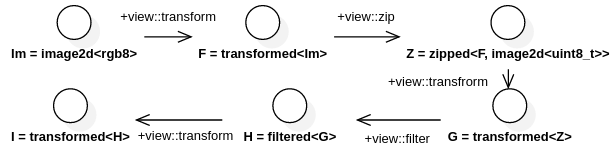
\includegraphics[height=2cm]{figs/viewAST.png}
  \caption{Abstract Syntax Tree of the types chained by the code above}
  \label{fig.viewAST}
\end{figure}

The concept of \emph{View} brought to us a fundamental issue when dealing with images: \blockquote{\emph{What is an
    image?}}. More precisely: should an image always be the owner of its data buffer? Should we have a shared ownership of
the data buffer between all the images using it? Then what happens when the data changes? The issue about the semantic
of an image is crucial but also very similar to the issue there is to differentiate a \emph{container} (such as
\texttt{std::vector}, that is to say the data buffer) and a \emph{view} on this container in the \emph{Ranges TS}.

From here we have considered two approaches. The first one is to have \emph{shared ownership} of the data buffer for the
image and its derived views. However this does not allow the differentiation between an already computed image and a
lazy image. To be able to make this differentiation is crucial in an \emph{Image Processing library} as we want to make
the most out of the data we already have and we do not want to compute data we do not need. Also, we cannot distinguish
when the \emph{copyability} property is required. This is the main reason why we did not adopt this approach.

The second one is to make the differentiation between a \emph{concrete image} which owns the data (like the standard
containers) and the \emph{views} that are lightweight cheap-to-copy objects. Not all \emph{concrete image} may be
\emph{copyable}, but all \emph{views} are. This is a very important property as it simplify greatly the reasoning when
performance is needed. It also enables us to have a library design similar to the standard library which the user is
familiar with and, why not, have standard algorithm and standard view work on our images types. All of these are the
main reason why we decided to adopt this design. Henceforth from now on the \emph{Image} concept is similar to the
\emph{View} concept from which we refines a \emph{ConcreteImage} concept that requires a specific behavior as it owns
data.


\vspace{1cm}

In~\cref{subsec.gen.concept}, we saw that what is truly important is the behavior: an algorithm will require its input
to be able to behave a certain way, and if those requirements are fulfilled, then the algorithm can be used with this
set of inputs. This enables non-standard type of image to be input in algorithms, providing they still behave correctly.
The way how we can check if the required behavior is satisfied is a new C++20 feature called \emph{concept} (the authors
show how to leverage them in~\cite{roynard.2019.rrpr}) that will not be presented in this paper. Additionally to
concepts, C++20 introduces a new library facility called \emph{ranges}~\cite{niebler.2018.deepranges} which includes a
non-owning lightweight container called \emph{views} whose design is very similar to that of \emph{morphers}, introduced
in Milena~\cite{levillain.2009.ismm,geraud.2012.hdr}. Views are completely transferable to the image processing world.
Also, views feature interesting properties that an image processing practitioner will find to his taste.

A view is a \emph{lightweight object} that behaves exactly the same as an image: let $V$ be a view of an image defined
on $\mathcal{D}$ then we have $\forall{p}\in\mathcal{D}, v = V(p)$. It can be a random generator that yields a random
number each time $V(p)$ is called; a proxy to the underlying image that records the number of times each pixel is
accessed in order, for instance, to compare algorithm performance; a projection to a specific color channel; applying an
automatic gamma correction; restricting the definition domain $\mathcal{D}$; and so on.

A view is a \emph{non-owning}, \emph{cheap-to-copy} lightweight object that basically only \emph{records an operation}
and stores a pointer to an image. For instance, let us consider the view transform defined as follow $v = transform(u_1,
  u_2, \cdots, u_n, f)$ where $u_i$ are input images and $h$ a n-ary function. $transform$ returns an image generated from
the other image(s) as show in~\cref{fig.view.threshold}. Also, we can see that the view itself does not own any image
but just stores pointers as well as the operation ($h$). This means that, for instance, modifying the original values of
the image(s) will impact the values yield by the view. Finally, as the view is cheap-to-copy, it features a pointer
semantic that help the practitioner passing around his images by copy to his algorithms without worrying about heavy
buffer copies in the background.

\begin{figure}[tbh]
  \centering
  \begin{minipage}{\linewidth}
    \includestandalone[mode=image, width=.9\linewidth]{figs/transform_thresholding}
  \end{minipage}
  \caption{An image view performing a thresholding.}
  \label{fig.view.threshold}
\end{figure}

Another key point of views is the lazy evaluation. When an image is piped through a view, no computation is done. The
computation happens when the practitioner requests a value by doing $val = V(p)$. The implications are multiples: an
image can be piped into several computation-heavy views, some of which can be discarded later on, it won't impact the
performance. Also, when processing large images, applying a transformation on a part of the image is as simple as
restricting the domain with a view and applying the transformation to this resulting sub-image.

Views will also try to preserve properties of the original image when they can. That means that views can preserve the
ability of the practitioner to, for instance, write into this image. This may be a trivial property to preserve when
considering a view that restrict a domain, but when considering a view that transforms the resulting values, it is not.
Let us consider the projection $h: (r,g,b) \mapsto g$ that selects the green component of an RGB triplet. When piping
the resulting view into, for instance, a blurring algorithm, the computation will take place in place thanks to still
having the ability to write into the image. A legacy way of obtaining the same result would have been to create a
temporary single-channel image consisting of the green channel of the original RGB image so that the temporary image
could then be blurred. Then one would have needed to copy the values of the temporary image back into the green channel
of the original image. The comparison between the legacy way and the in-place way of doing this computation is shown
in~\cref{fig.legacy.vs.view}.

\begin{figure}[tbh]
  \centering
  \subfloat[Legacy pipeline with copy]{
    \includegraphics[width=1.6in,align=t]{figs/blur_copy}
  }
  \hfil
  \subfloat[Modern pipeline with view]{
    \includegraphics[width=1.6in,align=t]{figs/blur_inplace}
  }

  \caption{Comparison of a legacy and a modern pipeline using \colorbox{lightgreen}{algorithms} and
    \colorbox{thistle}{views}.}
  \label{fig.legacy.vs.view}
\end{figure}

On the other hand, when considering the view $g: (r,g,b) \mapsto 0.2126*r+0.7152*g+0.0722*b$ that compute the gray level
of a color triplet (as shown in~\cref{fig.view.grayscale}), the ability to write a value into the image is not
preserved. One would need an inverse function that is able to deduce the original color triplet from the gray level to
be able to write back into the original image.

\begin{figure}[tbh]
  \centering
  \includegraphics[width=.98\linewidth]{figs/views/transform_grayscale}
  \caption{Usage of transform view: grayscale.}
  \label{fig.view.grayscale}
\end{figure}

\begin{figure}[tbh]
  \includestandalone[mode=image, scale=0.6]{figs/clip}

  \includestandalone[mode=image, scale=0.6]{figs/filter}
  \caption{Clip and filter image adaptors that restrict the image domain by a non-regular ROI and by a predicate that
    selects only even pixels.}
  \label{fig.view.clip}
\end{figure}

Following the same principle, a view can apply a restriction on an image domain. In~\cref{fig.view.clip}, we show the
adaptor \texttt{clip(input, roi)} that restricts the image to a non-regular \texttt{roi} and \texttt{filter(input,
  predicate)} that restricts the domain based on a predicate. All subsequent operations on those images will only affect
the selected pixels.

\begin{figure}[tbh]
  \includestandalone[mode=image, scale=0.6]{figs/pipeline}
  \caption{Example of a simple image processing pipeline.}
  \label{fig.view.pipeline}
\end{figure}

Views feature many interesting properties that change the way we program an image processing application. To illustrate
those features, let us consider the following image processing pipeline: (Start) Load an input RGB-8 2D image (a
classical HDR photography) (A) Convert it in grayscale (B) Sub-quantize to 8-bits (C) Perform the grayscale dilation of
the image (End) Save the resulting 2D 8-bit grayscale image; as described in~\cref{fig.view.pipeline}.


\begin{figure}[tbh]
  \begin{minipage}{\linewidth}
    \includestandalone[mode=image, scale=0.59]{figs/composition}
  \end{minipage}
  \caption{Algorithm vs image view composition.}
  \label{fig.view.comp}
\end{figure}

\textbf{Views are composable.} Chaining operations has always been a very important feature in image processing as well
as in software engineering in general (known object composition). Being able to weave simple blocks together into more
complex blocks in a way that the resulting block can still be treated as a simple block is a most wanted feature.
The~\cref{fig.view.pipeline} features an example of a pipeline using 3 basic operations \emph{Image} $\rightarrow$
\emph{Image}: a grayscale conversion, a sub-quantization and a dilation. It is important to note that we can consider
there is only one complex operation composed of 3 basic algorithms in which an image is piped. A view thus carries both
information about the image and the transformations. In~\cref{fig.view.comp} we show the distinction between the
composition of algorithms and the compositions of views which carry both the image and the transformations.

\textbf{Views improve usability.} The code featuring the pipeline in~\cref{fig.view.comp} can almost be implemented the
following way:
\begin{minted}{c++}
auto input = imread(...);
auto A = transform(input, [](rgb16 x) -> float {
    return (x.r + x.g + x.b) / 3.f; };
auto MyComplexImage = transform(A, [](float x)
    -> uint8_t { return (x / 256 + .5f); };
\end{minted}
When one is familiar to functional programming, it is quite easy to draw the parallel between \emph{transform},
\emph{map}, \emph{filter} and the sequence operators. Views are, in reality, higher-order functions built from an image
as well as the function(s) (operator or predicate) to apply for each pixel. It is not required to make the iteration
over each pixel of the image oneself, we just provide the function to morph the image into another one. The technique
used when composition several sequence operators is called \emph{currying}~\cite{hanus.1995.curry} in the functional
programming world.

\textbf{Views improve re-usability.} When looking at the code snippets above, one could see that they are simple though
not very re-usable. However, keeping the functional programming paradigm in mind, one can easily define new views just
by considering that a view is a \emph{higher-order function}. Then, as shown in~\cref{fig.view.highorder}, the primitive
\emph{transform} serves as the basis to build three new views: one that performs the summation of two images, one that
performs the grayscale conversion and one that performs the sub-quantization. All those three views can then be reused
afterwards\footnote{A more generic implementation could have been provided for these views for even more re-usability,
  but this is not the purpose here.}.

\begin{figure}
  \noindent
  \begin{minted}{c++}
auto operator+(Image A, Image B) {
  return transform(A, B, std::plus<>());
}
auto togray = [](Image A) { return transform(A, [](auto x)
  { return (x.r + x.g + x.b) / 3.f; };)
};
auto subquantize16to8b = [](Image A) { return transform(A,
  [](float x) { return uint8_t(x / 256 +.5f); });
};

auto input = imread(...);
auto MyComplexImage = subquantize16to8b(togray(A));
  \end{minted}

  \caption{Using high-order primitive views to create custom view operators.}
  \label{fig.view.highorder}
\end{figure}

\textbf{Views for lazy computing.} One fundamental point of views is that they embed the operation within themselves,
meaning that in~\cref{fig.view.highorder}, the creation of the views does not incur any computation. The computation is
delayed until the invocation of the \texttt{v(p)} expression. Also, the computation can be delayed quite far thanks to
the composition capability of views. In fact, a view is an image adaptor which actually is a \emph{template
  expression}~\citep{veldhuizen.1995.expression, veldhuizen.2000.blitz}. Indeed, the \emph{expression} used to generate
the image is recorded as a template parameter. A view is represented by an \emph{expression tree}, as shown
in~\cref{fig.view.ast}.


\begin{figure}
  \null\hfill
  \begin{minipage}[b]{2cm}
    \includestandalone[mode=image, scale=0.8]{figs/view_ast}
  \end{minipage}
  \begin{minipage}[b]{5.5cm}
    \begin{minted}{c++}
Image f = ...; // grayscale
Image g = ...; // rgb16
Image out = subquantize16to8b(
              togray(g)) + f;
\end{minted}
  \end{minipage}
  \caption{View composition seen as an expression tree.}
  \label{fig.view.ast}
\end{figure}



\PLAGIAT{
  \textbf{Views for performance.} Consider a classical design where each operation of the pipeline is implemented on
  ``its own''. Each operation requires that memory be allocated for the output image, and also, each operation requires
  that the image be traversed. This design is simple, flexible, composable, but is not memory efficient nor
  computationally efficient. With the lazy evaluation approach, the image is traversed only once (when the dilation is
  applied) that has two benefits. First, there are no intermediate images so this is memory effective. Second, it is
  faster thanks to a better memory cache usage; processing a RGB16 pixel from the dilation algorithm directly converts
  it in grayscale, then sub-quantized it to 8-bits, and finally make it available. It acts \emph{as if} we were writing
  an optimal operator that would combine these operations.
}

\PLAGIAT{
  As an experiment, we benchmarked both pipelines on a 20MPix image RGB16 (random generated values) on a desktop
  computer i7-2600 CPU @ 3.40GHz, single-threaded\footnote{Experimentation code is available at
    \url{https://gitlab.lrde.epita.fr/mroynard/roynard.icip.2020.snippets}}. The dilation is done with a small 3x3 square
  structuring element using tiling for caching input values. The pipeline using views is about 20\% faster than the
  regular one (133 vs 106 ms). Note that views are also compatible with optimizations such as parallelization and
  vectorization.
}

\PLAGIAT{
  Background Subtraction: The background subtraction pipeline is used to detect changes in image
  sequences~\cite{opencv.bg_sub}. It is mainly used when regions of interest are foreground objects. The pipeline
  components include: subtraction, Gaussian filtering, threshold, erode and dilate, as shown
  in~\cref{fig.view.comp.sub_bg}.
}

\begin{figure}[tbh]
  \begin{minipage}{\linewidth}
    \includestandalone[mode=image, scale=0.59]{figs/pipeline_bg_sub_comp}
  \end{minipage}
  \caption{Background substraction pipeline using \colorbox{lightgreen}{algorithms} and
    \colorbox{thistle}{views}.}
  \label{fig.view.comp.sub_bg}
\end{figure}


\clearpage


\begin{itemize}
  \item origine, parallèle avec range-v3
  \item Value/Ref semantics des images
  \item Comment préserver les propriétés
  \item Évaluation paresseuse
  \item Composabilité/chaînage
  \item ...
  \item Performances + Bench
\end{itemize}

\cleardoublepage


\part{Static-dynamic bridge}
\label{part.static_dynamic_bridge}

\begin{itemize}
  \item rappel de la problématique (backward ref depuis Généricité/4.)
  \item expliquer l'approche hybride (son design et les techniques de dispatch n*n avec variants)
  \item bench, trade-off
  \item continuité sur JIT avec autowig, cppyy (perspective)
\end{itemize}

\cleardoublepage


\part{Conclusion and perspectives}
\label{part.conclusion_and_perspecitves}


\begin{itemize}
  \item Synthèse générale
  \item Réponse à la problématique d'Introduction
  \item confrontation à d'autres travaux de recherche ayant donné naissance à une bibliothèque de TI
  \item Ouvertures, perspectives, limites
  \begin{itemize}
    \item continuité JIT
    \item ce qu'il reste à faire
  \end{itemize}
\end{itemize}

\cleardoublepage


\part{Appendices}
\label{part.annexes}

\appendix

\chapter{Bibliography}
\label{chap.bibliography}

\bibliographystyle{abbrv}
\bibliography{bibliography}

\chapter{Dynamic dispatch vs. Static dispatch in C++}
\label{appendix.dispatch.dyn.static}

The main advantage brought by using C++ as the implementation language for an image processing library is to be able to
leverage what is called metaprogramming. Metaprogramming is a way to tell the compiler to make decision about which
type, which code to generate. These decisions, made at compile time, and then absent from the resulting binary: only the
fast and optimised code remains. This bring a new distinction between the static world (what is decided at compile time)
and the dynamic world (what is decided at runtime). The more is decided at compile time the smaller, faster the binary
will because there is work less to do at runtime. By following this principle, one can think of some properties that are
known ahead of time (at compilation) when writing one's image processing algorithm. For instance, when considering the
example of the dilation whose code is shown in~\ref{fig.decomp.dilate}, we can see that the property about the
decomposability if the structuring element is linked to the type. This means that when the structuring element's type is
of a disc, or a square, the compiler will know at compile time that it is decomposable. To tell the compiler to take
advantage of a property at compile time, C++ has a language construct named if-constexpr. The resulting code then
becomes:

\begin{minted}[highlightlines=3]{c++}
  template <Image Img, StructuringElement SE>
  auto dilate(Img img, SE se) {
    if constexpr (se.is_decomposable()) {
      lst_small_se = se.decompose();
      for (auto small_se : lst_small_se)
        img = dilate(img, small_se) // Recursive call
      return img;
    } else if (is_pediodic_line(se))
      return fast_dilate1d(img, se) // Van Herk's algorithm;
    else
      return dilate_normal(img, se) // Classic algorithm;
  }
\end{minted}

There are other ways to achieve the same result with different language constructs in C++. There are two "legacy"
language construct which are tag dispatching (or overload) and SFINAE. With the release of C++17 came a new language
construct presented above: if-constexpr. Finally, with C++20, it will be possible to use concepts to achieve the same
result. To achieve the same result as above with tag dispatching, one would need to write the following code:

\begin{minted}[highlightlines={1-2,7,14}]{c++}
  struct SE_decomp {};
  struct SE_no_decomp {};

  template <Image Img, StructuringElement SE>
  auto dilate(Img img, SE se) {
    // either SE_decompo or SE_no_decomp
    return dilate_(img, se, typename SE::decomposable());
  }

  auto dilate_(Img img, SE se, SE_decomp) {
    lst_small_se = se.decompose();
    for (auto small_se : lst_small_se)
      // Recursive call
      img = dilate(img, small_se, SE_no_decomp)
    return img;
  }
  auto dilate_(Img img, SE se, SE_no_decomp) {
    if (is_pediodic_line(se))
      return fast_dilate1d(img, se) // Van Herk's algorithm;
    else
      return dilate_normal(img, se) // Classic algorithm;
  }
\end{minted}

To achieve the same result with SFINAE, one would need to write the following code:

\begin{minted}[highlightlines={5-6,14,23}]{c++}
  // SFINAE helper
  template <typename SE, typename = void>
  struct is_decomposable : std::false_type {};
  template <typename SE>
  struct is_decomposable<SE,
    // Check wether the type provides the decompose() method
    std::void_t<decltype(std::declval<SE>().decompose())>
  > : std::true_type {};
  template <typename SE>
  constexpr bool is_decomposable_v =
                  is_decomposable<SE>::value;

  template <Image Img, StructuringElement SE,
    typename = std::enable_if_t<is_decomposable_v<SE>>>
  auto dilate(Img img, SE se) {
    lst_small_se = se.decompose();
    for (auto small_se : lst_small_se)
      img = dilate(img, small_se) // Recursive call
    return img;
  }

  template <Image Img, StructuringElement SE,
    typename = std::enable_if_t<not is_decomposable_v<SE>>>
  auto dilate(Img img, SE se) {
    if (is_pediodic_line(se))
      return fast_dilate1d(img, se) // Van Herk's algorithm;
    else
      return dilate_normal(img, se) // Classic algorithm;
  }
\end{minted}

Comparing those two last ways of writing static code to the first one comes to an obvious conclusion: the if-constexpr
facility is much more readable and maintainable than the two legacy ways of doing it. Finally, there is still another way
to handle the issue and it is with C++20's concepts. The following code demonstrates how to leverage this language
construct:

\begin{minted}[highlightlines={1-4,15}]{c++}
  template <typename SE>
  concept SE_decomposable = requires (SE se) {
    se.decompose(); // this method must exist
  };

  template <typename Img, typename SE>
  auto dilate(Img img, SE se) {
   if (is_pediodic_line(se))
      return fast_dilate1d(img, se) // Van Herk's algorithm;
    else
      return dilate_normal(img, se) // Classic algorithm;
  }

  template <typename Img, typename SE>
    requires SE_decomposable<SE>
  auto dilate(Img img, SE se) {
    lst_small_se = se.decompose();
    for (auto small_se : lst_small_se)
      img = dilate(img, small_se) // Recursive call
    return img;
  }
\end{minted}
A best-match mechanic operates under the hood to select the function overload whose concept is the most specialized when
possible.

\chapter{Concepts \& archetypes}
\label{appendix.concepts.and.archetypes}

\section{Concepts}

\subsection{Index}

\begin{minted}{c++}
// Index
template <typename Idx>
concept Index = std::signed_integral<Idx>;
\end{minted}


\subsection{Value}

\begin{minted}{c++}
// Value
template <typename Val>
concept Value = std::semiregular<Val>;

// ComparableValue
template <typename RegVal>
concept ComparableValue =
  std::regular<RegVal>;

// OrderedValue
template <typename STORegVal>
concept OrderedValue =
  std::regular<STORegVal> &&
  std::totally_ordered<STORegVal>;
\end{minted}


\subsection{Point}

\begin{minted}{c++}
// Point
template <typename P>
concept Point =
  std::regular<P> &&
  std::totally_ordered<P>;
\end{minted}


\subsection{Pixel}

\begin{minted}{c++}
// Pixel
template <class Pix> concept Pixel =
std::is_base_of_v<mln::details::Pixel<Pix>, Pix> &&
  std::copy_constructible<Pix> &&
  std::move_constructible<Pix> &&
  requires {
    typename pixel_value_t<Pix>;
    typename pixel_reference_t<Pix>;
    typename pixel_point_t<Pix>;
  } &&
  std::semiregular<pixel_value_t<Pix>> &&
  Point<pixel_point_t<Pix>> &&
  !std::is_const_v<pixel_value_t<Pix>> &&
  !std::is_reference_v<pixel_value_t<Pix>> &&
  requires(const Pix cpix, Pix pix, pixel_point_t<Pix> p) {
    { cpix.point() } -> std::convertible_to<pixel_point_t<Pix>>;
    { cpix.val() }   -> std::convertible_to<pixel_reference_t<Pix>>;
    { pix.shift(p) };
  };

// WritablePixel
template <typename WPix>
concept WritablePixel =
  Pixel<WPix> &&
  requires(const WPix cpix, pixel_value_t<WPix> v) {
    // Not deep-const, view-semantic.
    { cpix.val() = v };
    // Proxy rvalues must not be deep-const on their assignement semantic (unlike tuple...)
    { const_cast<typename WPix::reference const &&>(cpix.val()) = v };
  };

// OutputPixel
template <typename Pix>
concept OutputPixel = detail::WritablePixel<Pix>;
\end{minted}


\subsection{Ranges}

\begin{minted}{c++}
template <class C>
concept MDCursor =
  std::ranges::detail::forward_cursor<C> &&
  std::ranges::detail::forward_cursor<std::ranges::detail::begin_cursor_t<C>> &&
  requires (C c)
  {
    { c.read() } -> std::ranges::forward_range;
    c.end_cursor();
  };

template <class C>
concept NDCursor = std::semiregular<C> &&
  requires (C c)
  {
    { C::rank } -> std::same_as<int>;
    c.read();
    c.move_to_next(0);
    c.move_to_end(0);
  };

template <class C>
concept MDBidirectionalCursor = MDCursor<C> &&
  requires (C c)
  {
    c.move_to_prev();
    c.move_to_prev_line();
  };

template <class R>
concept MDRange =
  requires(R r)
  {
    { r.rows() } -> std::ranges::forward_range;
    { r.begin_cursor() } -> MDCursor;
    { r.end_cursor() } -> std::same_as<std::ranges::default_sentinel_t>;
  };

template <class R>
concept MDBidirectionalRange = MDRange<R> &&
  requires (R r)
  {
    { r.rrows() } -> std::ranges::forward_range;
    { r.rbegin_cursor() } -> MDCursor;
    { r.rend_cursor() } -> std::same_as<std::ranges::default_sentinel_t>;
  };

template <class R>
concept mdrange = MDRange<R> || std::ranges::range<R>;

template <class R, class V>
concept output_mdrange = mdrange<R> && std::ranges::output_range<mdrange_row_t<R>, V>;

template <class R>
concept reversible_mdrange = MDBidirectionalRange<R> || std::ranges::bidirectional_range<R>;
\end{minted}


\subsection{Domain}

\begin{minted}{c++}
// Domain
template <typename Dom>
concept Domain =
  mln::ranges::mdrange<Dom> &&
  Point<mln::ranges::mdrange_value_t<Dom>> &&
  requires(const Dom cdom, mln::ranges::mdrange_value_t<Dom> p) {
    { cdom.has(p) }   -> std::same_as<bool>;
    { cdom.empty() }  -> std::same_as<bool>;
    { cdom.dim() }    -> std::same_as<int>;
  };


// SizedDomain
template <typename Dom>
concept SizedDomain =
  Domain<Dom> &&
  requires(const Dom cdom) {
    { cdom.size() } -> std::unsigned_integral;
  };

// ShapedDomain
template <typename Dom>
concept ShapedDomain =
  SizedDomain<Dom> &&
  requires(const Dom cdom) {
    { cdom.extents() }  -> std::ranges::forward_range;
  };
\end{minted}


\subsection{Extension}

\begin{minted}{c++}
template <typename Ext, typename Pnt>
concept Extension =
  std::is_base_of_v<mln::Extension<Ext>, Ext> &&
  requires {
    typename Ext::support_fill;
    typename Ext::support_mirror;
    typename Ext::support_periodize;
    typename Ext::support_clamp;
    typename Ext::support_extend_with;
  } &&
  Value<typename Ext::value_type> &&
  requires (const Ext cext,
      mln::archetypes::StructuringElement<
        Pnt,
        mln::archetypes::Pixel> se, const Pnt pnt) {
    { cext.fit(se) }      -> bool;
    { cext.extent() }     -> int;
  };

template <typename Ext>
concept FillableExtension =
  Extension<Ext> &&
  std::convertible_to<typename Ext::support_fill, std::true_type> &&
  requires {
    typename Ext::value_type;
  } &&
  requires (Ext ext, const Ext cext, const typename Ext::value_type& v) {
    { ext.fill(v) };
    { cext.is_fill_supported() }  -> bool;
  };

template <typename Ext>
concept MirrorableExtension =
  Extension<Ext> &&
  std::convertible_to<typename Ext::support_mirror, std::true_type> &&
  requires (Ext ext, const Ext cext, std::size_t padding) {
    { ext.mirror() };
    { ext.mirror(padding) };
    { cext.is_mirror_supported() }  -> bool;
  };

template <typename Ext>
concept PeriodizableExtension =
  Extension<Ext> &&
  std::convertible_to<typename Ext::support_periodize, std::true_type> &&
  requires (Ext ext, const Ext cext) {
    { ext.periodize() };
    { cext.is_periodize_supported() }  -> bool;
  };

template <typename Ext>
concept ClampableExtension =
  Extension<Ext> &&
  std::convertible_to<typename Ext::support_clamp, std::true_type> &&
  requires (Ext ext, const Ext cext) {
    { ext.clamp() };
    { cext.is_clamp_supported() }  -> bool;
  };

template <typename Ext, typename U>
concept ExtendWithExtension =
  Extension<Ext> &&
  std::convertible_to<typename Ext::support_extend_with, std::true_type> &&
  InputImage<U> &&
  requires {
    typename Ext::value_type;
    typename Ext::point_type;
  } &&
  std::convertible_to<typename U::value_type, typename Ext::value_type> &&
  std::convertible_to<typename Ext::point_type, typename U::point_type> &&
  requires (Ext ext, const Ext cext, U u, typename Ext::point_type offset) {
    { ext.extend_with(u, offset) };
    { cext.is_extend_with_supported() }  -> bool;
  };
\end{minted}


\subsection{Image}

\begin{minted}{c++}
template <typename I>
concept Image =
  // Minimum constraint on image object
  // Do not requires DefaultConstructible
  std::is_base_of_v<mln::details::Image<I>, I> &&
  std::copy_constructible<I> &&
  std::move_constructible<I> &&
  std::derived_from<image_category_t<I>, forward_image_tag> &&
  requires {
    typename image_pixel_t<I>;
    typename image_point_t<I>;
    typename image_value_t<I>;
    typename image_domain_t<I>;
    typename image_reference_t<I>;
    typename image_concrete_t<I>;
    typename image_ch_value_t<I, mln::archetypes::Value>;
    // traits
    typename image_indexable_t<I>;
    typename image_accessible_t<I>;
    typename image_extension_category_t<I>;
    typename image_category_t<I>;
    typename image_view_t<I>;
  } &&
  Pixel<image_pixel_t<I>> &&
  Point<image_point_t<I>> &&
  Value<image_value_t<I>> &&
  Domain<image_domain_t<I>> &&
  std::convertible_to<pixel_point_t<image_pixel_t<I>>, image_point_t<I>> &&
  std::convertible_to<pixel_reference_t<image_pixel_t<I>>, image_reference_t<I>> &&
  // Here we don't want a convertible constraint as value_type is the decayed type and should really be the same
  std::same_as<pixel_value_t<image_pixel_t<I>>, image_value_t<I>> &&
  std::common_reference_with<image_reference_t<I>&&, image_value_t<I>&> &&
  std::common_reference_with<image_reference_t<I>&&, image_value_t<I>&&> &&
  std::common_reference_with<image_value_t<I>&&, const image_value_t<I>&> &&
  requires(I ima, const I cima, image_domain_t<I> d, image_point_t<I> p) {
    { cima.template ch_value<mln::archetypes::Value>() }
        -> std::convertible_to<image_ch_value_t<I, mln::archetypes::Value>>;
    { cima.concretize() } -> std::convertible_to<image_concrete_t<I>>;
    { cima.domain() }     -> std::convertible_to<image_domain_t<I>>;
    { ima.pixels() }  -> mln::ranges::mdrange;
    { ima.values() }  -> mln::ranges::mdrange;
    requires std::convertible_to<mln::ranges::mdrange_value_t<decltype(ima.pixels())>, image_pixel_t<I>>;
    requires std::convertible_to<mln::ranges::mdrange_value_t<decltype(ima.values())>, image_value_t<I>>;
  };

namespace detail
{
  // WritableImage
  template <typename I>
  concept WritableImage =
    Image<I> &&
    OutputPixel<image_pixel_t<I>> &&
    requires(I ima) {
    { ima.values() }  -> mln::ranges::output_mdrange<image_value_t<I>>;
      // Check Writability of each pixel of the range
      requires OutputPixel<
                  std::common_type_t<
                    mln::ranges::mdrange_value_t<decltype(ima.pixels())>,
                    image_pixel_t<I>>>;
    };
} // namespace detail


// InputImage
template <typename I>
concept InputImage = Image<I>;


// ForwardImage
template <typename I>
concept ForwardImage = InputImage<I>;


// IndexableImage
template <typename I>
concept IndexableImage =
  Image<I> &&
  requires {
    typename image_index_t<I>;
  } &&
  image_indexable_v<I> &&
  requires (I ima, image_index_t<I> k) {
    { ima[k] }  -> std::same_as<image_reference_t<I>>; // For concrete image it returns a const_reference
  };


namespace detail
{
  // WritableIndexableImage
  template <typename I>
  concept WritableIndexableImage =
    WritableImage<I> &&
    IndexableImage<I> &&
    requires(I ima, image_index_t<I> k, image_value_t<I> v) {
      { ima[k] = v } -> std::same_as<image_reference_t<I>>;
    };
} // namespace detail

// AccessibleImage
template <typename I>
concept AccessibleImage =
  Image<I> &&
  image_accessible_v<I> &&
  requires (I ima, image_point_t<I> p) {
    { ima(p) }              -> std::same_as<image_reference_t<I>>; // For concrete image it returns a const_reference
    { ima.at(p) }           -> std::same_as<image_reference_t<I>>; // idem
    { ima.pixel(p) }    -> std::same_as<image_pixel_t<I>>; // For concrete image pixel may propagate constness
    { ima.pixel_at(p) } -> std::same_as<image_pixel_t<I>>; // idem
  };


namespace detail
{
  // WritableAccessibleImage
  template <typename I>
  concept WritableAccessibleImage =
    detail::WritableImage<I> &&
    AccessibleImage<I> &&
    requires(I ima, image_point_t<I> p, image_value_t<I> v) {
      { ima(p) = v };
      { ima.at(p) = v };
    };
} // namespace detail

// IndexableAndAccessibleImage
template <typename I>
concept IndexableAndAccessibleImage =
  IndexableImage<I> &&
  AccessibleImage<I> &&
  requires (const I cima, image_index_t<I> k, image_point_t<I> p) {
    { cima.point_at_index(k) }  -> std::same_as<image_point_t<I>>;
    { cima.index_of_point(p) }  -> std::same_as<image_index_t<I>>;
    { cima.delta_index(p) }     -> std::same_as<image_index_t<I>>;
  };


namespace detail
{
  // WritableIndexableAndAccessibleImage
  template <typename I>
  concept WritableIndexableAndAccessibleImage =
    IndexableAndAccessibleImage<I> &&
    detail::WritableImage<I> &&
    detail::WritableIndexableImage<I>;
} // namespace detail

// BidirectionalImage (not in STL term)
template <typename I>
concept BidirectionalImage =
  Image<I> &&
  std::derived_from<image_category_t<I>, bidirectional_image_tag> &&
  requires (I ima) {
  { ima.pixels() }  -> mln::ranges::reversible_mdrange;
  { ima.values() }  -> mln::ranges::reversible_mdrange;
};


namespace detail
{
  // WritableBidirectionalImage
  template <typename I>
  concept WritableBidirectionalImage =
    WritableImage<I> &&
    BidirectionalImage<I>;
} // namespace detail

// RawImage (not contiguous, stride = padding)
template <typename I>
concept RawImage =
  IndexableAndAccessibleImage<I> &&
  BidirectionalImage<I> &&
  std::derived_from<image_category_t<I>, raw_image_tag> &&
  requires (I ima, const I cima, int dim) {
    { ima.data() }        -> std::convertible_to<const image_value_t<I>*>; // data() may be proxied by a view
    { cima.stride(dim) } -> std::same_as<std::ptrdiff_t>;
  };


namespace detail
{
  // WritableRawImage
  template <typename I>
  concept WritableRawImage =
    WritableImage<I> &&
    WritableIndexableAndAccessibleImage<I> &&
    WritableBidirectionalImage<I> &&
    RawImage<I> &&
    requires(I ima, image_value_t<I> v) {
      { ima.data() }        -> std::convertible_to<image_value_t<I>*>;
      { *(ima.data()) = v };
    };
} // namespace detail


// OutputImage
// Usage: RawImage<I> && OutputImage<I>
template <typename I>
concept OutputImage =
  (not ForwardImage<I> || (detail::WritableImage<I>)) &&
  (not IndexableImage<I> || (detail::WritableIndexableImage<I>)) &&
  (not AccessibleImage<I> || (detail::WritableAccessibleImage<I>)) &&
  (not IndexableAndAccessibleImage<I> ||
    (detail::WritableIndexableAndAccessibleImage<I>)) &&
  (not BidirectionalImage<I> || (detail::WritableBidirectionalImage<I>)) &&
  (not RawImage<I> || (detail::WritableRawImage<I>));


template <typename I>
concept WithExtensionImage =
  Image<I> &&
  requires {
    typename image_extension_t<I>;
  } &&
  Extension<image_extension_t<I>> &&
  not ::std::same_as<mln::extension::none_extension_tag, image_extension_category_t<I>> &&
  requires (I ima, image_point_t<I> p) {
    { ima.extension() } -> ::std::convertible_to<image_extension_t<I>>;
  };


// ConcreteImage
template <typename I>
concept ConcreteImage =
  Image<I> &&
  std::semiregular<I> &&  // A concrete image is default constructible
  not image_view_v<I>;


// ViewImage
template <typename I>
concept ViewImage =
  Image<I> &&
  image_view_v<I>;
\end{minted}


\subsection{Structuring Element}

\begin{minted}{c++}
namespace details
{
  template <typename SE>
  concept DynamicStructuringElement =
    requires (SE se) {
    { se.radial_extent() }  -> std::same_as<int>;
    };


  constexpr bool implies(bool a, bool b) { return !a || b; }
}


template <typename SE, typename P>
concept StructuringElement =
  std::convertible_to<SE, mln::details::StructuringElement<SE>> &&
  std::ranges::regular_invocable<SE, P> &&
  std::ranges::regular_invocable<SE, mln::archetypes::PixelT<P>> &&
  requires {
    typename SE::category;
    typename SE::incremental;
    typename SE::decomposable;
    typename SE::separable;
  } &&
  std::convertible_to<typename SE::category, mln::adaptative_neighborhood_tag> &&
  details::implies(std::convertible_to<typename SE::category, mln::dynamic_neighborhood_tag>,
                    details::DynamicStructuringElement<SE>) &&
  requires (SE se, const SE cse, P p, mln::archetypes::PixelT<P> px) {
    { se(p) }         -> std::ranges::forward_range;
    { se(px) }        -> std::ranges::forward_range;
    { cse.offsets() } -> std::ranges::forward_range;

    requires std::convertible_to<std::ranges::range_value_t<decltype(se(p))>, P>;
    requires std::Pixel<std::ranges::range_value_t<decltype(se(px))>>;
    requires std::convertible_to<std::ranges::range_value_t<decltype(cse.offsets())>, P>;
  };

namespace details
{
  template <typename R, typename P>
  concept RangeOfStructuringElement =
    StructuringElement<std::ranges::range_value_t<R>, P>;
}



template <typename SE, typename P>
concept DecomposableStructuringElement =
  StructuringElement<SE, P> &&
  std::convertible_to<typename SE::decomposable, std::true_type> &&
  requires(const SE se) {
    { se.is_decomposable() }  -> std::same_as<bool>;
    { se.decompose() }        -> std::ranges::forward_range;
    requires details::RangeOfStructuringElement<decltype(se.decompose()), P>;
  };


template <typename SE, typename P>
concept SeparableStructuringElement =
  StructuringElement<SE, P> &&
  std::convertible_to<typename SE::separable, std::true_type> &&
  requires(const SE se) {
    { se.is_separable() } -> std::same_as<bool>;
    { se.separate() }     -> std::ranges::forward_range;
    requires details::RangeOfStructuringElement<decltype(se.separate()), P>;
  };


template <typename SE, typename P>
concept IncrementalStructuringElement =
  StructuringElement<SE, P> &&
  std::convertible_to<typename SE::incremental, std::true_type> &&
  requires(const SE se) {
    { se.inc() }  -> StructuringElement<P>;
    { se.dec() }  -> StructuringElement<P>;
  };
\end{minted}

\subsection{Neighborhood}

\begin{minted}{c++}
template <typename SE, typename P>
concept Neighborhood =
  StructuringElement<SE, P> &&
  requires (SE se, P p, mln::archetypes::PixelT<P> px) {
    { se.before(p) }  -> std::ranges::forward_range;
    { se.after(p) }   -> std::ranges::forward_range;
    { se.before(px) } -> std::ranges::forward_range;
    { se.after(px) }  -> std::ranges::forward_range;

    requires std::convertible_to<std::ranges::range_value_t<decltype(se.before(p))>, P>;
    requires std::convertible_to<std::ranges::range_value_t<decltype(se.after(p))>, P>;
    requires std::Pixel<std::ranges::range_value_t<decltype(se.before(px))>>;
    requires std::Pixel<std::ranges::range_value_t<decltype(se.after(px))>>;
  };
\end{minted}


\section{Archetypes}

\subsection{Index}

\begin{minted}{c++}
using Index = int;

static_assert(mln::concepts::Index<Index>, "Index archetype does not model the Index concept!");
\end{minted}


\subsection{Value}

\begin{minted}{c++}
struct Value
{
};

struct ComparableValue
{
};
bool operator==(const ComparableValue&, const ComparableValue&);
bool operator!=(const ComparableValue&, const ComparableValue&);


struct OrderedValue
{
};
bool operator==(const OrderedValue&, const OrderedValue&);
bool operator!=(const OrderedValue&, const OrderedValue&);
bool operator<(const OrderedValue&, const OrderedValue&);
bool operator>(const OrderedValue&, const OrderedValue&);
bool operator<=(const OrderedValue&, const OrderedValue&);
bool operator>=(const OrderedValue&, const OrderedValue&);

static_assert(mln::concepts::Value<Value>, "Value archetype does not model the Value concept!");
static_assert(mln::concepts::ComparableValue<ComparableValue>, "ComparableValue archetype does not model the ComparableValue concept!");
static_assert(mln::concepts::OrderedValue<OrderedValue>, "OrderedValue archetype does not model the OrderedValue concept!");
\end{minted}


\subsection{Point}

\begin{minted}{c++}
struct Point final
{
};

bool operator==(const Point&, const Point&);
bool operator!=(const Point&, const Point&);
bool operator<(const Point&, const Point&);
bool operator>(const Point&, const Point&);
bool operator<=(const Point&, const Point&);
bool operator>=(const Point&, const Point&);

static_assert(mln::concepts::Point<Point>, "Point archetype does not model the Point concept!");
\end{minted}


\subsection{Pixel}

\begin{minted}{c++}
namespace details
{
  template <class P, class V>
  struct PixelT
  {
    using value_type = V;
    using point_type = P;
    using reference  = const value_type&;

    PixelT()              = delete;
    PixelT(const PixelT&) = default;
    PixelT(PixelT&&)      = default;
    PixelT& operator=(const PixelT&) = delete;
    PixelT& operator=(PixelT&&) = delete;

    point_type point() const;
    reference  val() const;
    void       shift(const P& dp);
  };

  struct OutputPixel : PixelT<Point, Value>
  {
    using reference = Value&;
    reference val() const;
  };


  template <class Pix>
  struct AsPixel : Pix, mln::details::Pixel<AsPixel<Pix>>
  {
  };
} // namespace details

template <class P, class V = Value>
using PixelT      = details::AsPixel<details::PixelT<P, V>>;
using Pixel       = PixelT<Point, Value>;
using OutputPixel = details::AsPixel<details::OutputPixel>;

static_assert(mln::concepts::Pixel<Pixel>, "Pixel archetype does not model the Pixel concept!");
static_assert(mln::concepts::OutputPixel<OutputPixel>, "OutputPixel archetype does not model the OutputPixel concept!");
\end{minted}


\subsection{Ranges}

\begin{minted}{c++}
  // TODO
\end{minted}


\subsection{Domain}

\begin{minted}{c++}
struct Domain
{
  using value_type = Point;
  using reference  = Point&;

  value_type* begin();
  value_type* end();

  bool has(value_type) const;
  bool empty() const;
  int  dim() const;
};

static_assert(mln::concepts::Domain<Domain>, "Domain archetype does not model the Domain concept!");

struct SizedDomain : Domain
{
  unsigned size() const;
};

static_assert(mln::concepts::SizedDomain<SizedDomain>,
                          "SizedDomain archetype does not model the SizedDomain concept!");

struct ShapedDomain final : SizedDomain
{
  static constexpr std::size_t  ndim = 1;
  value_type                    shape() const;
  std::array<std::size_t, ndim> extents() const;
};

static_assert(mln::concepts::ShapedDomain<ShapedDomain>,
                          "ShapedDomain archetype does not model the ShapedDomain concept!");
\end{minted}


\subsection{Extension}

\begin{minted}{c++}
  // TODO
\end{minted}


\subsection{Image}

\begin{minted}{c++}
namespace details
{
  template <class I>
  struct AsImage : I, mln::details::Image<AsImage<I>>
  {
    using I::I;

    using concrete_type = AsImage<typename I::concrete_type>;
    concrete_type concretize() const;


    template <typename V>
    using ch_value_type = AsImage<typename I::template ch_value_type<V>>;

    template <typename V>
    ch_value_type<V> ch_value() const;
  };


  struct ConcreteImage
  {
    using pixel_type = archetypes::Pixel;
    using value_type     = pixel_value_t<mln::archetypes::Pixel>;
    using reference      = pixel_reference_t<mln::archetypes::Pixel>;
    using point_type     =  std::ranges::range_value_t<Domain>;
    using domain_type    = Domain;
    using category_type  = forward_image_tag;
    using concrete_type  = ConcreteImage;

    template <class V>
    using ch_value_type = ConcreteImage;

    // additional traits
    using extension_category = mln::extension::none_extension_tag;
    using indexable          = std::false_type;
    using accessible         = std::false_type;
    using view               = std::false_type;

    ConcreteImage()                     = default;
    ConcreteImage(const ConcreteImage&) = default;
    ConcreteImage(ConcreteImage&&)      = default;
    ConcreteImage& operator=(const ConcreteImage&) = default;
    ConcreteImage& operator=(ConcreteImage&&) = default;

    domain_type domain() const;


    struct pixel_range
    {
      const pixel_type* begin();
      const pixel_type* end();
    };
    pixel_range pixels();


    struct value_range
    {
      const value_type* begin();
      const value_type* end();
    };

    value_range values();
  };


  struct ViewImage : ConcreteImage
  {
    using view = std::true_type;

    ViewImage()                 = delete;
    ViewImage(const ViewImage&) = default;
    ViewImage(ViewImage&&)      = default;
    ViewImage& operator=(const ViewImage&) = delete;
    ViewImage& operator=(ViewImage&&) = delete;
  };

  using Image = ViewImage;


  struct OutputImage : Image
  {
    using pixel_type = archetypes::OutputPixel;
    using reference      = pixel_reference_t<mln::archetypes::OutputPixel>;

    struct pixel_range
    {
      const pixel_type* begin();
      const pixel_type* end();
    };

    pixel_range pixels();

    struct value_range
    {
      value_type* begin();
      value_type* end();
    };

    value_range values();
  };


  struct OutputIndexableImage : OutputImage
  {
    using index_type = int;
    using indexable  = std::true_type;

    using concrete_type = OutputIndexableImage;

    template <class V>
    using ch_value_type = OutputIndexableImage;

    reference operator[](index_type);
  };


  struct IndexableImage : Image
  {
    using index_type = int;
    using indexable  = std::true_type;

    using concrete_type = OutputIndexableImage;

    template <class V>
    using ch_value_type = OutputIndexableImage;


    reference operator[](index_type);
  };

  struct OutputAccessibleImage : OutputImage
  {
    using accessible    = std::true_type;
    using concrete_type = OutputAccessibleImage;

    template <class V>
    using ch_value_type = OutputAccessibleImage;


    reference      operator()(point_type);
    reference      at(point_type);
    pixel_type pixel(point_type);
    pixel_type pixel_at(point_type);
  };


  struct AccessibleImage : Image
  {
    using accessible    = std::true_type;
    using concrete_type = OutputAccessibleImage;

    template <class V>
    using ch_value_type = OutputAccessibleImage;

    reference      operator()(point_type);
    reference      at(point_type);
    pixel_type pixel(point_type);
    pixel_type pixel_at(point_type);
  };


  struct OutputIndexableAndAccessibleImage : OutputAccessibleImage
  {
    using index_type = int;
    using indexable  = std::true_type;

    using concrete_type = OutputIndexableAndAccessibleImage;

    template <class V>
    using ch_value_type = OutputIndexableAndAccessibleImage;


    reference  operator[](index_type);
    point_type point_at_index(index_type) const;
    index_type index_of_point(point_type) const;
    index_type delta_index(point_type) const;
  };


  struct IndexableAndAccessibleImage : AccessibleImage
  {
    using index_type = int;
    using indexable  = std::true_type;

    using concrete_type = OutputIndexableAndAccessibleImage;

    template <class V>
    using ch_value_type = OutputIndexableAndAccessibleImage;

    reference  operator[](index_type);
    point_type point_at_index(index_type) const;
    index_type index_of_point(point_type) const;
    index_type delta_index(point_type) const;
  };


  struct BidirectionalImage : Image
  {
    using category_type = bidirectional_image_tag;

    struct pixel_range
    {
      const pixel_type* begin();
      const pixel_type* end();
      pixel_range           reversed();
    };

    pixel_range pixels();

    struct value_range
    {
      const value_type* begin();
      const value_type* end();
      value_range       reversed();
    };

    value_range values();
  };


  struct OutputBidirectionalImage : BidirectionalImage
  {
    using pixel_type = archetypes::OutputPixel;
    using reference      = pixel_reference_t<mln::archetypes::OutputPixel>;

    struct value_range
    {
      value_type* begin();
      value_type* end();
      value_range reversed();
    };
    value_range values();


    struct pixel_range
    {
      const pixel_type* begin();
      const pixel_type* end();
      pixel_range           reversed();
    };

    pixel_range pixels();
  };


  struct RawImage : IndexableAndAccessibleImage
  {
    using category_type = raw_image_tag;
    using pixel_range   = BidirectionalImage::pixel_range;
    using value_range   = BidirectionalImage::value_range;

    pixel_range pixels();
    value_range values();


    const value_type* data() const;
    std::ptrdiff_t    strides(int) const;
  };


  struct OutputRawImage : OutputIndexableAndAccessibleImage
  {
    using category_type = raw_image_tag;
    using pixel_range   = OutputBidirectionalImage::pixel_range;
    using value_range   = OutputBidirectionalImage::value_range;

    pixel_range pixels();
    value_range values();

    value_type*    data() const;
    std::ptrdiff_t strides(int) const;
  };


  struct WithExtensionImage : Image
  {
    struct Extension
    {
      // FIXME
    };

    using extension_type = Extension;

    using extension_category = mln::extension::custom_extension_tag;

    extension_type extension() const;
  };
} // namespace details


using Image         = details::AsImage<details::Image>;
using ConcreteImage = details::AsImage<details::ConcreteImage>;
using ViewImage     = details::AsImage<details::ViewImage>;

using ForwardImage       = Image;
using BidirectionalImage = details::AsImage<details::BidirectionalImage>;
using RawImage           = details::AsImage<details::RawImage>;

using InputImage                  = Image;
using IndexableImage              = details::AsImage<details::IndexableImage>;
using AccessibleImage             = details::AsImage<details::AccessibleImage>;
using IndexableAndAccessibleImage = details::AsImage<details::IndexableAndAccessibleImage>;


using OutputImage              = details::AsImage<details::OutputImage>;
using OutputForwardImage       = OutputImage;
using OutputBidirectionalImage = details::AsImage<details::OutputBidirectionalImage>;
using OutputRawImage           = details::AsImage<details::OutputRawImage>;

using OutputIndexableImage              = details::AsImage<details::OutputIndexableImage>;
using OutputAccessibleImage             = details::AsImage<details::OutputAccessibleImage>;
using OutputIndexableAndAccessibleImage = details::AsImage<details::OutputIndexableAndAccessibleImage>;

using WithExtensionImage = details::AsImage<details::WithExtensionImage>;
\end{minted}


\subsection{Structuring Element}

\begin{minted}{c++}
namespace details
{
  template <class P, class Pix>
  requires mln::concepts::Point<P>&& mln::concepts::Pixel<Pix>
  struct StructuringElement
  {
    using category     = adaptative_neighborhood_tag;
    using incremental  = std::false_type;
    using decomposable = std::false_type;
    using separable    = std::false_type;

     std::ranges::subrange<P*> operator()(P p);

     std::ranges::subrange<Pix*> operator()(Pix px);
     std::ranges::subrange<P*>   offsets() const;
  };


  template <class SE>
  struct AsSE : SE, mln::details::Neighborhood
  helper<AsSE<SE>>
  {
  };
} // namespace details

template <class P = Point, class Pix = PixelT<P>>
using StructuringElement = details::AsSE<details::StructuringElement<P, Pix>>;


namespace details
{
  template <class P, class Pix>
  struct DecomposableStructuringElement : StructuringElement<P, Pix>
  {
    using decomposable = std::true_type;

    bool                                                                is_decomposable() const;
    std::ranges::subrange<mln::archetypes::StructuringElement<P, Pix>*> decompose() const;
  };

  template <class P, class Pix>
  struct SeparableStructuringElement : StructuringElement<P, Pix>
  {
    using separable = std::true_type;

    bool                                                                is_separable() const;
    std::ranges::subrange<mln::archetypes::StructuringElement<P, Pix>*> separate() const;
  };

  template <class P, class Pix>
  struct IncrementalStructuringElement : StructuringElement<P, Pix>
  {
    using incremental = std::true_type;

    archetypes::StructuringElement<P, Pix> inc() const;
    archetypes::StructuringElement<P, Pix> dec() const;
  };
} // namespace details


template <class P = Point, class Pix = PixelT<P>>
using DecomposableStructuringElement = details::AsSE<details::DecomposableStructuringElement<P, Pix>>;

template <class P = Point, class Pix = PixelT<P>>
using SeparableStructuringElement = details::AsSE<details::SeparableStructuringElement<P, Pix>>;

template <class P = Point, class Pix = PixelT<P>>
using IncrementalStructuringElement = details::AsSE<details::IncrementalStructuringElement<P, Pix>>;
\end{minted}


\subsection{Neighborhood}

\begin{minted}{c++}
namespace details
{
  template <class P, class Pix>
  requires mln::concepts::Point<P>&& mln::concepts::Pixel<Pix>
  struct Neighborhood : StructuringElement<P, Pix>
  {
     std::ranges::iterator_range<P*>   before(P p);
     std::ranges::iterator_range<P*>   after(P p);
     std::ranges::iterator_range<Pix*> before(Pix px);
     std::ranges::iterator_range<Pix*> after(Pix px);
  };


  template <class N>
  struct AsNeighborhood : N, mln::details::Neighborhood<AsNeighborhood<N>>
  {
  };

} // namespace details

template <class P = Point, class Pix = PixelT<P>>
using Neighborhood = details::AsSE<details::Neighborhood<P, Pix>>;
\end{minted}


\end{document}
